\cleardoublepage

\newrefsection
\sectionmajornumbering

\chapter{外文翻译}
\title{局部间断伽辽金法分析半导体设备漂移扩散模型}
\author{刘蕴贤,舒其望}
\date{}
\maketitle
\sectionnonum{摘要}
在本文中,我们研究了一维半导体器件的漂移扩散(DD)模型,这是一个系统,不仅涉及一阶导数对流项,还涉及二阶导数扩散项和耦合的泊松电位方程。对于具有平滑解的半离散和全离散的局部间断伽罗华金(LDG)方案,获得了最优误差估计。在全离散方案中,我们将隐式-显式(IMEX)时间离散化与LDG空间离散化相结合,以允许更大的时间步长并节省计算成本。分析中的主要技术难点是处理由于数值方法的间断性以及模型的非线性和耦合性而产生的元素间跳跃项。我们还进行了模拟以验证分析。

\section{文献综述}
在之前的工作\parencite{liu2010errorc}中,我们已经分析了用于解决半导体器件模拟中时间依赖和稳态矩模型的局部间断伽辽金(LDG)有限元方法。在该方法中,同时存在一阶导数对流项和二阶导数扩散(热传导)项,并且对流-扩散系统通过局部不连续 Galerkin (LDG) 方法进行离散化\parencite{cockburn1998local,cockburn2001runge},也可以参考\parencite{bank1983numerical,bank1998finite,chainais2003finite,bessemoulin2012finite}。

在工作\parencite{liu2010errorc}中,我们仅使用LDG方法对电子浓度方程进行离散化。对于电势方程,我们仍然使用连续方法,以避免在单元边界上出现两个独立解变量的不连续性,这样很难进行分析。此外,由于电子浓度和电场的非线性耦合,当在LDG方案中使用$P^k$元(分段多项式,次数为k)时,我们仅获得了次优误差估计$O(h^{k+\frac{1}{2}})$。

在本文中,我们将给出半离散LDG格式与隐式-显式(IMEX)时间离散化LDG格式(参见\parencite{wang2015stability,wang2015stabilityd})用于光滑解的误差估计。
与\parencite{liu2010errorc}中的情况不同的是,本文中的势能方程也通过LDG方法进行离散化。
通过使用LDG方法进行统一离散化,可以充分实现该方法在简单h-p自适应性和并行效率方面的潜力。
\parencite{liu2004local,liu2007locala}中展示的数值结果已经表明,对于矩模型,这种统一的LDG离散化表与与ENO有限差分方法\parencite{jerome1994energy}的结果相比表现良好。
然而,据我们所知,直到现在还没有针对这种统一方法的误差估计。在完离散格式中,我们将LDG格式与1-3阶精度的IMEX龙格-库塔时间离散化耦合。
我们显式处理非线性耦合项,隐式处理扩散项。通过这种处理,我们证明IMEX LDG方案是无条件稳定的,即使非线性耦合项是显式处理的。
通过允许我们使用更大的时间步长,这极大地提高了该方案的计算效率。

现在我们简要回顾LDG方法的背景。LDG方法具有几个吸引人的特点\parencite{xu2010local}。它们可以轻松地设计为任何精度。实际上,精度的阶数可以在每个单元中进行局部确定,这允许高效的p自适应性。它们可以用于任意三角剖分,甚至包括具有悬挂节点(不同单元共享的节点,但具有不同属性)的三角剖分,这样可以实现高效的h自适应性。
这些方法具有出色的并行效率,因为它们在本质上是非常局部的,每个单元只需要与其直接相邻的单元进行通信,而不受精度的影响。此外,这些方法具有优秀的可证明非线性稳定性。

对于解决线性守恒律平滑解的DG方法,\parencite{richter1988optimalordera,meng2015optimal,lesaint1974finite,johnson1986analysisa,cockburn2008optimala}给出了对于张量积和某些特殊网格的优化先验误差估计$O(h^{k+1})$,对于其他情况给出了$O(h^{k+\frac{1}{2}})$的估计。Cockburn和Shu\parencite{cockburn1998local}首次得到了线性对流-扩散方程LDG方法的先验误差估计。之后,Castillo等人\parencite{castillo2000optimala,castillo2000priorib,castillo2002optimalb}证明了使用特定数值通量的LDG方法的收敛阶数O(hk+1)的最优性。Rivi`ere和Wheeler\parencite{cockburn2000development}给出了至少对于二次多项式的非线性对流-扩散方程方法的最优误差估计。Zhang和Shu在\parencite{zhang2004errorc,zhang2006errorb,zhang2010stabilitya,luo2015priori}中给出了针对标量非线性守恒律和可对称系统的完全离散Runge-Kutta DG方法的先验误差估计,参见Burman、Ern和Fern ́andez \parencite{burman2010explicit}。Xu和Shu\parencite{xu2007errora}给出了针对非线性对流-扩散方程和具有平滑解的KdV方程的半离散局部不连续Galerkin方法的L2误差估计。Wang、Shu和Zhang\parencite{wang2015stability,wang2015stabilityd}得到了应用于线性和非线性对流-扩散问题的LDG方法与IMEX时间步进的最优误差估计。

尽管LDG方法已经进行有了许多理论分析,但对于涉及与泊松势方程耦合的半导体器件矩模型的分析,通过统一LDG方法对浓度方程和势能方程进行处理,似乎还没有可用的分析结果。主要困难在于如何处理两个独立解变量(一个来自浓度方程,另一个来自势能方程)在单元间的不连续问题。
通过探索数值解的梯度与接口跳跃之间的重要关系,并结合LDG方法中梯度的独立数值解,我们在本文中得到了半离散LDG方案和IMEX LDG方案的最优误差估计。

本文的结构如下所述。第2节列出了一些预备知识。第3节介绍了漂移扩散(DD)模型并给出了其弱形式。第4节给出了具有周期边界条件的DD模型的半离散LDG格式及其误差估计。第5节包含了具有周期边界条件的DD模型的几个IMEX LDG格式及其误差估计。第6节得到了具有Dirichlet边界条件的DD模型的LDG方案的误差估计。第7节呈现了模拟结果。第8节给出了总结和未来工作计划。
\section{预备知识}
本节将介绍一些符号定义并提供一些辅助结论。
首先使有限元空间的基础符号。然后定义具体的投影并提供特定的插值和有限元空间的逆性质。
\subsection{基础符号}
$I_j = (x_{j-\frac{1}{2}},x_{j+\frac{1}{2}}),j=1,2,\cdots,N$是计算域I的一个划分。$\Delta x_j = x_{j+\frac{1}{2}}-x_{j-\frac{1}{2}},x_j = \frac{1}{2}(x_{j-\frac{1}{2}}+x_{j+\frac{1}{2}}), h = \max\{\sup\limits_{j} \Delta x_j\}$。
有限维计算空间
\begin{equation*}
    V_h = V_h^k = \{z:z|_{I_j} \in P^k(I_j)\}
\end{equation*}
其中$P^k(I_j)$表示定义在$I_j$上维数不大于k的多项式集。数值解和测试函数都来至空间$V_h^k$。
在$V_h^k$中,函数允许在接口$x_{j+\frac{1}{2}}$跳跃间断,因此$V_h^k \not\subseteq H^1$,其中$H^k = W^{k,2}$,后者表示Sobolev空间。这时DG法和其他有限元方法的主要区别。而且网格大小$\Delta x_j$和多项式阶k可以随着单位元自由改变,这允许h-p自适应性。h-adaptivity(网格自适应),p-adaptivity(多项式自适应)。
定义$(u_h)^+_{j+\frac{1}{2}} = u_h(x^+_{j+\frac{1}{2}})$和$(u_h)^-_{j+\frac{1}{2}} = u_h(x^-_{j+\frac{1}{2}})$。用$[u_h]_{j+\frac{1}{2}} = (u_h)^+_{j+\frac{1}{2}} - (u_h)^-_{j+\frac{1}{2}}$和$(\bar{u}_h)_{j+\frac{1}{2}}=\frac{1}{2}((u_h)^+_{j+\frac{1}{2}}+(u_h)^-_{j+\frac{1}{2}})$来表示$u_h$在每个单元边界点的跳跃和平均值。

C是与h无关的正常数,可能依赖于PDE的准确解。$\tilde{\epsilon}$表示小的正常数。两者每次出现可能取不同的值。在本文的讨论的问题中,准确解被假定为光滑的。另外$0\leq t \leq T$,因此,准确解恒有界。
\subsection{投影和插值性质}
我们考虑关于具有k+1阶连续导数u到空间$V_h^k$的标准$L^2$-投影$\mathcal{P}$,i.e.,对于每个j
\begin{equation}
    \int_{I_j}(\mathcal{P}u(x) - u(x))v(x)\rm{d} x = 0, \forall v \in P^k(I_j).
\end{equation}
到$V_h^k$的特殊投影$\mathcal{P}^{\pm}$满足对每个j
\begin{align}
    \int_{I_j}(\mathcal{P}^+u(x) - u(x))v(x)\rm{d} x = 0, \forall v \in P^{k-1}(I_j), \\
    \mathcal{P}^+u(x_{j-\frac{1}{2}}^+) = u(x_{j-\frac{1}{2}})\nonumber
\end{align}
和
\begin{align}
    \int_{I_j}(\mathcal{P}^-u(x) - u(x))v(x)\rm{d} x = 0, \forall v \in P^{k-1}(I_j), \\
    \mathcal{P}^-u(x_{j+\frac{1}{2}}^-) = u(x_{j+\frac{1}{2}}).\nonumber
\end{align}
利用上述性质可以得到
\begin{equation}
    ||\eta|| + h||\eta||_{0,\infty} + h^{\frac{1}{2}}||\eta||_{\Gamma_h} \leq Ch^{k+1},
\end{equation}
其中$\eta = \mathcal{P}u - u$或$\eta = \mathcal{P}^{\pm}u - u$。$||\dot||$表示$L^2$范数,$||\dot||_{0,\infty}$表示$L^{\infty}$范数和$||\eta||_{\Gamma_h} = [\sum_{j=1}^{N}((\eta_{j+\frac{1}{2}}^+)^2 + (\eta_{j+\frac{1}{2}}^-)^2)]^{\frac{1}{2}}$。正常数C仅依赖于u,与h无关。$\Gamma_h$表示说有单位元$I_j$的边界点的集合。
\subsection{逆性质}
最后,我们会理出一些有限元空间$V_h^k$逆性质(见\parencite{ciarlet1978finite}),它们将会用于我们的误差分析。
对于任意$v \in V_h^k$,存在与v和h无关的正常数$C_i$使得
\begin{equation}
    ||v_x|| \leq C_1 h^{-1} ||v||, \qquad
    ||v||_{\Gamma_h} \leq C_2 h^{-\frac{1}{2}}||v||, \qquad
    ||v||_{0,\infty} \leq C_3 h^{-\frac{d}{2}}||v||.
\end{equation}
其中d是空间维数。在我们的例子中d=1。
\section{漂移-扩散DD模型和弱形式}
\subsection{DD模型}
漂移-扩散模型由以下方程表示
\begin{align}
    n_t - (\mu En)_x = \tau \theta n_{xx}, \label{equation:DD:translation} \\
    \phi_{xx} = \frac{e}{\epsilon}(n - n_d),  \label{equation:poisson:translation}
\end{align}

其中$x \in (0,1)$,第一个方程具有周期边界条件,势方程具有Dirichlet边界条件:$\phi(0,t) = 0, \phi(1,t) = v_{bias}$。我们会在第六节考虑关于第一个方程的Dirichlet边界条件。泊松方程\eqref{equation:poisson:translation}是电势方程,$E = -\phi_x$代表电场。

在系统\eqref{equation:DD:translation}-\eqref{equation:poisson:translation},未知变量是电子浓度n和电势$\phi$。$m_0$是电子有效质量,k是Boltzmann常数,e是电子电荷,$\mu$是迁移率,$T_0$是晶格温度,$\tau = \frac{m_0 \mu}{e}$是松弛参数,$\theta = \frac{k}{m_0}T_0$,$\epsilon$是介电常量,$n_d$是掺杂,这是一个给定的函数。
\subsection{弱形式}
LDG法的出发点是引入一个辅助变量,将包含高阶空间导数的PDE\eqref{equation:DD:translation}改写为只包含一阶空间导数的更大系统。

令$q = \sqrt{\tau \theta }n_x$,因此等式\eqref{equation:DD:translation}可以写作
\begin{align}
    n_t - (\mu E n)_x - \sqrt{\tau \theta}q_x = 0, \\
    q - \sqrt{\tau \theta}n_x = 0,                 \\
    E_x = -\frac{e}{\epsilon}(n - n_d),            \\
    E = - \phi_x.
\end{align}
我们用测试函数$v,w,r,z \in V_h^k$分别乘以上述方程,再对所有包含空间导数的部分进行公式化的分部积分来得到
\begin{align}
    \int_{I_j} n_t v \rm{d}x + \int_{I_j}(\mu En + \sqrt{\tau \theta}q)v_x\rm{d} x          \nonumber                                                                                                                         \\
    - (\mu En + \sqrt{\tau \theta}q)_{j+\frac{1}{2}}v_{j+\frac{1}{2}}^- +(\mu En + \sqrt{\tau \theta}q)_{j-\frac{1}{2}}v_{j-\frac{1}{2}}^+ = 0, \label{weakForm:1:translation}                                                \\
    \int_{I_j} qw\rm{d}x + \int_{I_j}\sqrt{\tau \theta} n w_x \rm{d}x - \sqrt{\tau \theta} n_{j+\frac{1}{2}}w_{j+\frac{1}{2}}^- + \sqrt{\tau \theta} n_{j-\frac{1}{2}}w_{j-\frac{1}{2}}^+ = 0, \label{weakForm:2:translation} \\
    -\int_{I_j}Er_x\rm{d}x + E_{j+\frac{1}{2}}r_{j+\frac{1}{2}}^- - E_{j-\frac{1}{2}}r_{j-\frac{1}{2}}^+ = -\frac{e}{\epsilon}\int_{I_j}(n-n_d)r\rm{d}x,                                       \label{weakForm:3:translation} \\
    \int_{I_j} Ez \rm{d}x - \int_{I_j}\phi z_x \rm{d}x + \phi_{j+\frac{1}{2}}z_{j+\frac{1}{2}}^- - \phi_{j-\frac{1}{2}}z_{j-\frac{1}{2}}^+ = 0,\label{weakForm:4:translation}
\end{align}
其中$ j=1,\cdots,N$,$v,w,r,z \in V_h$。

\section{半离散LDG格式其误差估计}
\subsection{半离散LDG格式}
将上述方程中的精确解$n,q,E,\phi$替换为数值近似$n_h,q_h,E_h,\phi_h \in V_h^k$,注意到数值解$n_h,q_h,E_h,\phi_h$在单元边界处不连续,然后用合适的数值通量来替换单元边界的项,我们得到半离散LDG法:对于任意的$t>0$,找数值解$n_h,q_h,E_h,\phi_h \in V_h$使得
\begin{align}
    \int_{I_j} (n_h)_t v \rm{d}x + \int_{I_j}(\mu E_h n_h + \sqrt{\tau \theta}q_h)v_x\rm{d} x                                                               \nonumber                                                                             \\
    - (\mu E_hn_h + \sqrt{\tau \theta}\hat{q}_h)_{j+\frac{1}{2}}v_{j+\frac{1}{2}}^- +(\mu \hat{E_hn_h} + \sqrt{\tau \theta}\hat{q}_h)_{j-\frac{1}{2}}v_{j-\frac{1}{2}}^+ = 0,                                   \label{LDG:1:translation}         \\
    \int_{I_j} q_hw \rm{d}x + \int_{I_j}\sqrt{\tau \theta} n_h w_x \rm{d}x - \sqrt{\tau \theta} (\hat{n}_h)_{j+\frac{1}{2}}w_{j+\frac{1}{2}}^- + \sqrt{\tau \theta} (\hat{n}_h)_{j-\frac{1}{2}}w_{j-\frac{1}{2}}^+ = 0, \label{LDG:2:translation} \\
    -\int_{I_j}E_hr_x\rm{d}x + (\hat{E}_h)_{j+\frac{1}{2}}r_{j+\frac{1}{2}}^- - (\hat{E}_h)_{j-\frac{1}{2}}r_{j-\frac{1}{2}}^+ = -\frac{e}{\epsilon}\int_{I_j}(n_h-n_d)r\rm{d}x,                                        \label{LDG:3:translation} \\
    \int_{I_j} E_hz \rm{d}x - \int_{I_j}\phi_h z_x \rm{d}x + (\hat{\phi}_h)_{j+\frac{1}{2}}z_{j+\frac{1}{2}}^- - (\hat{\phi}_h)_{j-\frac{1}{2}}z_{j-\frac{1}{2}}^+ = 0,\label{LDG:4:translation}
\end{align}
其中$ j=1,\cdots,N$,$v,w,r,z \in V_h$。

带“帽”的项是数值通量。 我们选择通量$\hat{E_h n_h} = \frac{1}{2}((E_hn_h)^+  + (E_hn_h)^-)$,$\hat{n}_h$和$\hat{q}_h$的交变通量,即
\begin{equation}
    \hat{n}_h = (n_h)^+, \hat{q}_h = (q_h)^- \quad \text{or} \quad \hat{n}_h = (n_h)^-, \hat{q}_h = (q_h)^+, \label{numbericalFlux:n&q:translation}
\end{equation}
$\hat{\phi}_h$和$\hat{E}_h$的交变通量,带有一个边界条件的调节来考虑Dirichlet边界条件,即
\begin{equation}
    \begin{aligned}
        (\hat{\phi}_h)_{\frac{1}{2}} = (\phi_h^-)_{\frac{1}{2}} = 0, (\hat{\phi}_h)_{j-\frac{1}{2}} = (\phi_h^+)_{j-\frac{1}{2}},j = 2,\cdots,N,(\hat{\phi}_h)_{N-\frac{1}{2}} = (\phi_h^+)_{N-\frac{1}{2}} = v_{bias}, \\
        (\hat{E_h})_{\frac{1}{2}} = (E_h^+)_{\frac{1}{2}} + c_0[\phi]_{\frac{1}{2}}, (\hat{E}_h)_{j-\frac{1}{2}} = (E_h^-)_{j-\frac{1}{2}} + c_0[\phi]_{j-\frac{1}{2}},j = 2,\cdots,N+1,
    \end{aligned}\label{numbericalFlux:phi&E:translation}
\end{equation}
或
\begin{equation}
    \begin{aligned}
        (\hat{\phi}_h)_{\frac{1}{2}} = (\phi_h^-)_{\frac{1}{2}} = 0, (\hat{\phi}_h)_{j-\frac{1}{2}} = (\phi_h^-)_{j-\frac{1}{2}},j = 2,\cdots,N,(\hat{\phi}_h)_{N-\frac{1}{2}} = (\phi_h^+)_{N-\frac{1}{2}} = v_{bias}, \\
        (\hat{E_h})_{j - \frac{1}{2}} = (E_h^+)_{j - \frac{1}{2}} + c_0[\phi]_{j-\frac{1}{2}},j = 2,\cdots,N, (\hat{E}_h)_{N+\frac{1}{2}} = (E_h^-)_{N+\frac{1}{2}} + c_0[\phi]_{N+\frac{1}{2}}.
    \end{aligned}\label{numbericalFlux:phi&E alt:translation}
\end{equation}
注意辅助变量$q_h$和$E_h$可以从\eqref{weakForm:2:translation}或\eqref{weakForm:4:translation}中解出并且带入\eqref{weakForm:1:translation}或\eqref{weakForm:3:translation}。这就是这种方法被叫做“局部”不连续Galerkin法的原因,同时也区分LDG法和经典混合有限元方法的原因。后者的辅助变量$q_h$或$E_h$必须从全局系统中求出。

\subsection{误差估计}
在下面关于半离散法的分析中定义$||u||_{L^{\infty}(0,T;L^2)}  = \max \limits_{0 \leq t \leq T}||u||_{l^2(I)}$和$||u||_{L^2(0,T;L^2)} = (\int_{0}^{T}||u||_{L^2(I)}^2\rm{d}t)^{\frac{1}{2}}$。
\begin{theorem}
    令n,q为问题\eqref{weakForm:1:translation}-\eqref{weakForm:4}的精确解,且足够光滑,导数有界。令$n_h,q_h$为半离散LDG法\eqref{LDG:1:translation}-\ref{LDG:4}的数值解。定义对应的数值误差$e_u = u - u_h (u = n,q)$。如果有限元空间$V_h^k$是间断$k(k\geq 0)$阶多形式,那么队医足够小的h,存在下列误差估计
    \begin{equation}
        ||n - n_h||_{L^{\infty}(0,T;L^2)} + ||q - q_h||_{L^2(0,T;L^2)} \leq C h^{k+1},
    \end{equation}
    其中常数C依赖于最终时间T,k,反常数$C_2$,$||n||_{L^{\infty}(0,T;L^2)}$,$||n_x||_{L^{\infty}}$和$||E||_{L^{\infty}}$。
\end{theorem}

在证明定理之前,我们首先给出两个引理。
\begin{lemma}
    设 $E$ 是问题(3.9)-(3.10)的精确解, $E_{h}$ 是半离散 LDG 方案(4.3)-(4.4)的数值解。我们有
    \begin{equation}
        \left\|E-E_{h}\right\| \leq C\left(h^{k+1}+\left\|n-n_{h}\right\|\right).
    \end{equation}
    对于定周期边界条件的这个引理的详细证明,我们参见\parencite{ayuso2011discontinuous}。对于我们的情况,即对$\phi$的狄里克雷边界条件,可以沿着类似的线索进行证明,因此这里不再给出。
\end{lemma}

我们回顾一下,我们已经选择了交错的通量$\hat{n}_{h}$和$\hat{q}_{h}$,即$\hat{n}_{h}=\left(n_{h}\right)^{+}$,$\hat{q}_{h}=\left(q_{h}\right)^{-}$。我们将误差$e_{u}=u-u_{h}(u=n, q)$写为$e_{u}=\xi_{u}-\eta_{u}$,其中$\xi_{n}=\mathcal{P}^{+} n-n_{h}$,$\eta_{n}=\mathcal{P}^{+} n-n ; \xi_{q}=\mathcal{P}^{-} q-q_{h}, \eta_{q}=\mathcal{P}^{-} q-q$。然后我们声明第二个引理:

\begin{lemma}
    \begin{align}
         & \left\|\xi_{n, x}\right\| \leq \frac{C_{\mu}}{\sqrt{\tau \theta}}\left(\left\|\xi_{q}\right\|+\left\|\eta_{q}\right\|\right)                      \\
         & \left|\sqrt{h^{-1}}\left[\xi_{n}\right]\right| \leq \frac{C_{\mu}}{\sqrt{\tau \theta}}\left(\left\|\xi_{q}\right\|+\left\|\eta_{q}\right\|\right)
    \end{align}
    对此引理的详细证明,我们参考\parencite{wang2015stability}。
\end{lemma}
\begin{proof}
    定理4.1的证明: 考虑方程(3.7)和(4.1)的差异,以及方程(3.8)和(4.2)的差异,我们得到以下误差方程
    \begin{align}
         & \int_{I_{j}}\left(n-n_{h}\right)_{t} v d x+\int_{I_{j}} \mu\left(E n-E_{h} n_{h}\right) v_{x} d x                                                                                                                                       \nonumber \\
         & -\mu\left(E n-\widehat{E_{h} n_{h}}\right)_{j+\frac{1}{2}} v_{j+\frac{1}{2}}^{-}+\mu\left(E n-\widehat{E_{h} n_{h}}\right)_{j-\frac{1}{2}} v_{j-\frac{1}{2}}^{+}                                                                        \nonumber \\
         & +\int_{I_{j}} \sqrt{\tau \theta}\left(q-q_{h}\right) v_{x} d x-\sqrt{\tau \theta}\left(q-\hat{q}_{h}\right)_{j+\frac{1}{2}} v_{j+\frac{1}{2}}^{-}+\sqrt{\tau \theta}\left(q-\hat{q}_{h}\right)_{j-\frac{1}{2}} v_{j-\frac{1}{2}}^{+}=0 .          \\
         & \quad \int_{I_{j}}\left(q-q_{h}\right) w d x+\int_{I_{j}} \sqrt{\tau \theta}\left(n-n_{h}\right) w_{x} d x                                                                                                                              \nonumber \\
         & \quad-\sqrt{\tau \theta}\left(n-\hat{n}_{h}\right)_{j+1 / 2} w_{j+\frac{1}{2}}^{-}+\sqrt{\tau \theta}\left(n-\hat{n}_{h}\right)_{j-1 / 2} w_{j-\frac{1}{2}}^{+}=0 .
    \end{align}
    如果我们在误差方程(4.12)-(4.13)中选择 $v=\xi_{n}$ 和 $w=\xi_{q}$,我们得到:
    \begin{equation}
        \begin{aligned}
             & \int_{I_{j}}\left(n-n_{h}\right)_{t} v d x+\int_{I_{j}} \mu\left(E n-E_{h} n_{h}\right) v_{x} d x                                                                                                                                        \\
             & -\mu\left(E n-\widehat{E_{h} n_{h}}\right)_{j+\frac{1}{2}} v_{j+\frac{1}{2}}^{-}+\mu\left(E n-\widehat{E_{h} n_{h}}\right)_{j-\frac{1}{2}} v_{j-\frac{1}{2}}^{+}                                                                         \\
             & +\int_{I_{j}} \sqrt{\tau \theta}\left(q-q_{h}\right) v_{x} d x-\sqrt{\tau \theta}\left(q-\hat{q}_{h}\right)_{j+\frac{1}{2}} v_{j+\frac{1}{2}}^{-}+\sqrt{\tau \theta}\left(q-\hat{q}_{h}\right)_{j-\frac{1}{2}} v_{j-\frac{1}{2}}^{+}=0 . \\
             & \quad \int_{I_{j}}\left(q-q_{h}\right) w d x+\int_{I_{j}} \sqrt{\tau \theta}\left(n-n_{h}\right) w_{x} d x                                                                                                                               \\
             & \quad-\sqrt{\tau \theta}\left(n-\hat{n}_{h}\right)_{j+1 / 2} w_{j+\frac{1}{2}}^{-}+\sqrt{\tau \theta}\left(n-\hat{n}_{h}\right)_{j-1 / 2} w_{j-\frac{1}{2}}^{+}=0 .
        \end{aligned}
    \end{equation}
    和
    \begin{equation}
        \begin{split}
            & \int_{I_{j}}\left(\xi_{q}-\eta_{q}\right) \xi_{q} d x+\int_{I_{j}} \sqrt{\tau \theta}\left(\xi_{n}-\eta_{n}\right) \xi_{q, x} d x                                                                \\
            & -\sqrt{\tau \theta}\left(\xi_{n}-\eta_{n}\right)_{j+\frac{1}{2}}^{+} \xi_{q, j+\frac{1}{2}}^{-}+\sqrt{\tau \theta}\left(\xi_{n}-\eta_{n}\right)_{j-\frac{1}{2}}^{+} \xi_{q, j-\frac{1}{2}}^{+}=0
        \end{split}
    \end{equation}
    将上述两个方程相加,并对 $j$ 求和,我们得到:
    \begin{equation}
        \begin{split}
            & \sum_{j=1}^{N} \int_{I_{j}} \xi_{n, t} \xi_{n} d x+\sum_{j=1}^{N} \int_{I_{j}} \xi_{q}^{2} d x \\
            = & \sum_{j=1}^{N} \int_{I_{j}} \eta_{n, t} \xi_{n} d x+\sum_{j=1}^{N} \int_{I_{j}} \eta_{q} \xi_{q} d x \\
            + & \sum_{j=1}^{N}\left(\int_{I_{j}} \sqrt{\tau \theta} \eta_{q} \xi_{n, x} d x+\int_{I_{j}} \sqrt{\tau \theta} \eta_{n} \xi_{q, x} d x-\sqrt{\tau \theta} \eta_{q, j+\frac{1}{2}}^{-} \xi_{n, j+\frac{1}{2}}^{-}\right. \\
            & \left.+\sqrt{\tau \theta} \eta_{q, j-\frac{1}{2}}^{-} \xi_{n, j-\frac{1}{2}}^{+}-\sqrt{\tau \theta} \eta_{n, j+\frac{1}{2}}^{+} \xi_{q, j+\frac{1}{2}}^{-}+\sqrt{\tau \theta} \eta_{n, j-\frac{1}{2}}^{+} \xi_{q, j-\frac{1}{2}}^{+}\right) \\
            + & \sum_{j=1}^{N}\left(-\int_{I_{j}} \sqrt{\tau \theta} \xi_{q} \xi_{n, x} d x-\int_{I_{j}} \sqrt{\tau \theta} \xi_{n} \xi_{q, x} d x+\sqrt{\tau \theta} \xi_{q, j+\frac{1}{2}}^{-} \xi_{n, j+\frac{1}{2}}^{--}\right. \\
            & \left.-\sqrt{\tau \theta} \xi_{q, j-\frac{1}{2}}^{-} \xi_{n, j-\frac{1}{2}}^{+}+\sqrt{\tau \theta} \xi_{n, j+\frac{1}{2}}^{+} \xi_{q, j+\frac{1}{2}}^{-}-\sqrt{\tau \theta} \xi_{n, j-\frac{1}{2}}^{+} \xi_{q, j-\frac{1}{2}}^{+}\right) \\
            + & \sum_{j=1}^{N}\left(-\int_{I_{j}} \mu\left(E n-E^{h} n^{h}\right) \xi_{n, x} d x\right. \\
            & \left.+\mu\left(E n-\widehat{E^{h} n^{h}}\right)_{j+\frac{1}{2}} \xi_{n, j+\frac{1}{2}}^{-}-\mu\left(E n-\widehat{E^{h} n^{h}}\right)_{j-\frac{1}{2}} \xi_{n, j-\frac{1}{2}}^{+}\right) \\
            = & T_{1}+T_{2}+T_{3}+T_{4}+T_{5} .
        \end{split}
    \end{equation}
    接下来,我们逐项估计 $T_{i}$。通过使用投影的性质(2.3)和Schwartz不等式,我们得到:
    \begin{align}
        T_{1}=\sum_{j=1}^{N} \int_{I_{j}} \eta_{n, t} \xi_{n} d x \leq C \int_{I} \eta_{n, t}^{2} d x+C \int_{I} \xi_{n}^{2} d x \leq C h^{2 k+2}+C\left\|\xi_{n}\right\|^{2} . \\
        T_{2}=\sum_{j=1}^{N} \int_{I_{j}} \eta_{q} \xi_{q} d x \leq C \int_{I} \eta_{q}^{2} d x+\tilde{\varepsilon} \int_{I} \xi_{q}^{2} d x \leq C h^{2 k+2}+\tilde{\varepsilon}\left\|\xi_{q}\right\|^{2} .
    \end{align}
    很显然,从投影(2.2)我们有:
    $$
        \int_{I_{j}} \eta_{n} v(x) d x=0, \quad \int_{I_{j}} \eta_{q} v(x) d x=0, \quad \forall v \in P^{k-1}\left(I_{j}\right),
    $$
    和 $\eta_{q, j+\frac{1}{2}}^{-}=0, \quad \eta_{n, j+\frac{1}{2}}^{+}=0$, 然后我们得到
    \begin{equation}
        T_{3}=0
    \end{equation}
    我们也有:
    \begin{equation}
        \begin{split}
            T_{4}= & \sum_{j=1}^{N}\left(-\int_{I_{j}} \sqrt{\tau \theta}\left(\xi_{q} \xi_{n}\right)_{x} d x+\sqrt{\tau \theta} \xi_{q, j+\frac{1}{2}}^{-} \xi_{n, j+\frac{1}{2}}^{-}\right.                                                                  \\
            & \left.-\sqrt{\tau \theta} \xi_{q, j-\frac{1}{2}}^{-} \xi_{n, j-\frac{1}{2}}^{+}+\sqrt{\tau \theta} \xi_{n, j+\frac{1}{2}}^{+} \xi_{q, j+\frac{1}{2}}^{-}-\sqrt{\tau \theta} \xi_{n, j-\frac{1}{2}}^{+} \xi_{q, j-\frac{1}{2}}^{+}\right)  \\
            =      & \sum_{j=1}^{N}\left(\sqrt{\tau \theta}\left(\xi_{q} \xi_{n}\right)_{j-\frac{1}{2}}^{+}-\sqrt{\tau \theta}\left(\xi_{q} \xi_{n}\right)_{j+\frac{1}{2}}^{-}+\sqrt{\tau \theta} \xi_{q, j+\frac{1}{2}}^{-} \xi_{n, j+\frac{1}{2}}^{-}\right. \\
            & \left.-\sqrt{\tau \theta} \xi_{q, j-\frac{1}{2}}^{-} \xi_{n, j-\frac{1}{2}}^{+}+\sqrt{\tau \theta} \xi_{n, j+\frac{1}{2}}^{+} \xi_{q, j+\frac{1}{2}}^{-}-\sqrt{\tau \theta} \xi_{n, j-\frac{1}{2}}^{+} \xi_{q, j-\frac{1}{2}}^{+}\right)  \\
            =      & \sum_{j=1}^{N} \sqrt{\tau \theta}\left(\xi_{n, j+1 / 2}^{+} \xi_{q, j+1 / 2}^{-}-\xi_{n, j-1 / 2}^{+} \xi_{q, j-1 / 2}^{-}\right)=0 .
        \end{split}
    \end{equation}
    上述估计使用了 $n, n_{h}, q$ 和 $q_{h}$ 的周期边界条件。关于(4.16)的最后一项 $T_{5}$,由于我们选择了 $\widehat{E_{h} n_{h}}=\frac{1}{2}\left(\left(E_{h} n_{h}\right)^{+}+\left(E_{h} n_{h}\right)^{-}\right)$,我们有:
    \begin{equation}
        T_{5}=-\int_{I} \mu\left(E n-E_{h} n_{h}\right) \xi_{n, x} d x-\sum_{j=1}^{N} \mu\left(E n-\frac{1}{2}\left(\left(E_{h} n_{h}\right)^{+}+\left(E_{h} n_{h}\right)^{-}\right)\right)_{j-\frac{1}{2}}\left[\xi_{n}\right]_{j-1 / 2}
    \end{equation}
    对于 $T_{5}$ 的积分部分,我们将其分为以下两部分处理:
    $$
        -\int_{I} \mu\left(E n-E_{h} n_{h}\right) \xi_{n, x} d x=-\int_{I} \mu E\left(n-n_{h}\right) \xi_{n, x} d x-\int_{I} \mu\left(E-E_{h}\right) n_{h} \xi_{n, x} d x
    $$
    目前,我们做出以下先验假设:
    \begin{equation}
        \left\|n-n_{h}\right\| \leq \tilde{C} h
    \end{equation}
    我们稍后会验证这个先验假设的合理性。这个先验假设意味着 $\left|n_{h}\right|{L^{\infty}} \leq C$。利用Young不等式,(2.3)和引理4.2,我们有:
    \begin{equation}
        \int_{I} \mu\left(E n-E_{h} n_{h}\right) \xi_{n, x} d x \leq C\left\|\xi_{n}\right\|^{2}+C h^{2 k+2}+\tilde{\varepsilon}\left\|\xi_{n, x}\right\|^{2}
    \end{equation}
    对于 $T{5}$ 的边界部分,我们有:
    $$
        \begin{aligned}
              & -\sum_{j=1}^{N} \mu\left(E n-\frac{1}{2}\left(\left(E_{h} n_{h}\right)^{+}+\left(E_{h} n_{h}\right)^{-}\right)\right)_{j-\frac{1}{2}}\left[\xi_{n}\right]_{j-1 / 2}                                                                                                                                              \\
            = & -\sum_{j=1}^{N} \mu\left(\frac{1}{2} E\left(n-\left(n_{h}\right)^{+}\right)+\frac{1}{2}\left(E-\left(E_{h}\right)^{+}\right)\left(n_{h}\right)^{+}\right.                                                                                                                                                        \\
              & \left.+\frac{1}{2} E\left(n-\left(n_{h}\right)^{-}\right)+\frac{1}{2}\left(E-\left(E_{h}\right)^{-}\right)\left(n_{h}\right)^{-}\right)_{j-\frac{1}{2}}\left[\xi_{n}\right]_{j-1 / 2}                                                                                                                            \\
            = & -\frac{1}{2} \sum_{j=1}^{N} \mu E_{j-\frac{1}{2}}\left(\xi_{n}^{+}+\xi_{n}^{-}-\eta_{n}^{+}-\eta_{n}^{-}\right)_{j-\frac{1}{2}}\left[\xi_{n}\right]_{j-1 / 2}                                                                                                                                                    \\
              & -\frac{1}{2} \sum_{j=1}^{N} \mu\left(E-\left(E_{h}\right)^{+}\right)_{j-\frac{1}{2}}\left(n_{h}\right)_{j-\frac{1}{2}}^{+}\left[\xi_{n}\right]_{j-1 / 2}-\frac{1}{2} \sum_{j=1}^{N} \mu\left(E-\left(E_{h}\right)^{-}\right)_{j-\frac{1}{2}}\left(n_{h}\right)_{j-\frac{1}{2}}^{-}\left[\xi_{n}\right]_{j-1 / 2}
        \end{aligned}
    $$
    利用Young不等式和 $\left|n_{h}\right|_{L^{\infty}} \leq C$,我们得到: $$
        \begin{aligned}
                 & -\sum_{j=1}^{N} \mu\left(E n-\frac{1}{2}\left(\left(E_{h} n_{h}\right)^{+}+\left(E_{h} n_{h}\right)^{-}\right)\right)_{j-\frac{1}{2}}\left[\xi_{n}\right]_{j-1 / 2}             \\
            \leq & C h\left(\left\|\xi_{n}\right\|_{\Gamma}^{2}+\left\|\eta_{n}\right\|_{\Gamma}^{2}+\left\|E-E_{h}\right\|_{\Gamma}^{2}\right)+\tilde{\varepsilon} h^{-1}\left[\xi_{n}\right]^{2}
        \end{aligned}
    $$
    然后从反性质(2.4),结合(4.9),我们可以得到
    \begin{equation}
        -\sum_{j=1}^{N} \mu\left(E n-\frac{1}{2}\left(\left(E_{h} n_{h}\right)^{+}+\left(E_{h} n_{h}\right)^{-}\right)\right)_{j-\frac{1}{2}}\left[\xi_{n}\right]_{j-1 / 2} \leq C\left(h^{2 k+2}+\left\|\xi_{n}\right\|^{2}\right)+\tilde{\varepsilon} h^{-1}\left[\xi_{n}\right]^{2}
    \end{equation}
    将(4.23)和(4.24)代入(4.21),我们有:
    \begin{equation}
        T_{5} \leq C\left\|\xi_{n}\right\|^{2}+C h^{2 k+2}+\tilde{\varepsilon}\left\|\xi_{n, x}\right\|^{2}+\tilde{\varepsilon} h^{-1}\left[\xi_{n}\right]^{2} .
    \end{equation}
    将(4.17)-(4.20)和(4.25)代入(4.16),我们得到:
    \begin{equation}
        \frac{1}{2} \frac{d}{d t}\left\|\xi_{n}\right\|^{2}+\left\|\xi_{q}\right\|^{2} \leq C\left\|\xi_{n}\right\|^{2}+C h^{2 k+2}+\tilde{\varepsilon}\left\|\xi_{n, x}\right\|^{2}+\tilde{\varepsilon} h^{-1}\left[\xi_{n}\right]^{2}+\tilde{\varepsilon}\left\|\xi_{q}\right\|^{2}
    \end{equation}
    利用引理4.3,以及投影的性质和Gronwall不等式,我们可以得到定理的结论。

    为了完成证明,让我们验证先验假设(4.22)的合理性。对于 $k \geq 0$,我们可以考虑 $h$ 足够小,使得 $C h^{k+1} \leq \frac{1}{2} \tilde{C} h$,其中 $C$ 是由最终时间 $T$ 确定的常数。然后如果 $t^* = \sup \left\{t:\left|n(t)-n_{h}(t)\right| \leq \tilde{C} h\right\}$,我们应该有 $\left|n\left(t^{}\right)-n_{h}\left(t^{}\right)\right|=\tilde{C} h$,如果 $t^{}$ 是有限的。另一方面,我们的证明意味着(4.8)对于 $t \leq t^{}$ 成立,特别地,$\left|n\left(t^{}\right)-n_{h}\left(t^{}\right)\right| \leq C h^{k+1} \leq \frac{1}{2} \tilde{C} h$。这是一个矛盾,如果 $t^* < T$。因此$t^* \geq T$,那么假设(4.22)就有效了。
\end{proof}

\section{IMEX RK全离散LDG格式和其误差估计}
在本节我们会考虑LDG空间离散化与[1,27]中提出的三阶特定IMEX龙格-库塔法相耦合。其想法是隐性处理线性扩散部分,显性处理非线性耦合漂移项来节省计算成本,同时依然追求无条件稳定性,即时间步长可以取小于给定常数的任意值。
\subsection{全离散法}
令$\{t^m = m\Delta t\}^M_{m = 0}$是时间区间[0,T]的均匀分割,时间步长为$\Delta t$。时间步长实际上可以一步步变化,但是在本文中我们为了简化取时间步长为常数。给定$n_h^m$,因此得到$q_h^m,E_h^m,\phi_h^m$,我们想找到在下一时间级别$t^{m+1}$处找到数值解,可以通过几个中间阶段$t^{m,l}$,通过下面IMEX RK法来实现。

\noindent \textbf{一阶格式}

使用一阶IMEX时间推进方案的LDG法,其中浓度方程中耦合的非线性部分用向前欧拉法处理,漂移部分用向后欧拉法处理,由以下形式给出:找到数值解$n_h^{m+1},q_h^{m+1}\in V_h$使得
\begin{align}
    (\frac{n_h^{m+1} - n_h^m}{\Delta t},v)_{I_j} & = -(\mu E_h^mn_h^m, v_x)_{I_j} + (\mu \hat{E_h^mn_h^m})_{j+\frac{1}{2}}v_{j-\frac{1}{2}}^- - (\mu\hat{E_h^mn_h^m})_{j-\frac{1}{2}}v^+_{j-\frac{1}{2}}                                         \nonumber                               \\
                                                 & -(\sqrt{\tau \theta}q_h^{m+1},v_x)_{I_j} + (\sqrt{\tau \theta}\hat{q}_h^{m+1})_{j+\frac{1}{2}}v_{j+\frac{1}{2}}^- - (\sqrt{\tau \theta}\hat{q}_h^{m+1})_{j-\frac{1}{2}}v_{j-\frac{1}{2}}^+,  \label{weakForm:IMEX1 LDG 1:translation} \\
    (q_h^{m+1},w)_{I_j}                          & = -(\sqrt{\tau \theta}n_h^{m+1},w_x)_{I_j} + (\sqrt{\tau \theta}\hat{n}_h^{m+1})_{j+\frac{1}{2}}w_{j+\frac{1}{2}}^- - (\sqrt{\tau \theta}\hat{n}_h^{m+1})_{j-\frac{1}{2}}w_{j-\frac{1}{2}}^+,\label{weakForm:IMEX1 LDG 2:translation}
\end{align}
其中$j = 1,\cdots,N;\quad r,z \in V_h$。

电势方程的LDG格式是:找到$E_h^{m},\phi_h^{m} \in V_h$,使得
\begin{align}
    -\int_{I_j} E_h^{m}r_x \rm{d}x + (\hat{E}_h^{m})_{j+\frac{1}{2}}r_{j+\frac{1}{2}}^- - (\hat{E}_h^{m})_{j-\frac{1}{2}}r_{j-\frac{1}{2}}^+ = -\frac{e}{\epsilon}\int_{I_j}(n_h^{m} - n_d) r\rm{d} x, \label{equation:IMEX1 LDG:EPE 1:translation} \\
    \int_{I_j} E_h^{m}z \rm{d}x - \int_{I_j} \phi_h^{m}z_x \rm{d}x  + (\hat{\phi}_h^{m})_{j+\frac{1}{2}}z^-_{j+\frac{1}{2}} - (\hat{\phi}_h^{m})_{j-\frac{1}{2}}z_{j-\frac{1}{2}}^+  = 0,\label{equation:IMEX1 LDG:EPE 2:translation}
\end{align}
中$j = 1,\cdots,N;\quad r,v \in V_h$并且$l = 0,1, u^{m,0} = u^m$。

与半离散情况相同,“hat”项是数值通量,依然选择为\eqref{numbericalFlux:n&q:translation}和\eqref{numbericalFlux:phi&E:translation}(或\eqref{numbericalFlux:phi&E alt:translation})。

\noindent \textbf{二阶格式}

因为二阶和三阶格式有许多项,为了简化符号,我们将定义
\begin{align}
    H_j(E_h,n_h,v) = - (\mu E_h n_h, v_x)_{I_j} + (\mu \hat{E_h n_h})_{j+\frac{1}{2}}v_{j+\frac{1}{2}}^- - (\mu \hat{E_h n_h})_{j-\frac{1}{2}}v_{j-\frac{1}{2}}^+, \label{notation:IMEX2 RK 1:translation} \\
    H_j^{\pm}(u_h,v) =- \sqrt{\tau \theta}(u_h,v_x)_{I_j} + \sqrt{\tau\theta}(u_h^{\pm})_{j+\frac{1}{2}}v_{j+\frac{1}{2}}^0 - \sqrt{\tau\theta}(u_h^{\pm})_{j-\frac{1}{2}}v_{j-\frac{1}{2}}^+,\quad u = n,q.\label{notation:IMEX2 RK 2:translation}
\end{align}
显然对于光滑的$E,n,u$我们有
\begin{align*}
    H_j(E,n,v) = -(\mu En,v_x)_{I_j} + (\mu En)_{j+\frac{1}{2}}v_{j+\frac{1}{2}}^- - (\mu En)_{j-\frac{1}{2}}v_{j-\frac{1}{2}}^+, \\
    H_j(E,n,v)^{\pm} = - \sqrt{\tau\theta}(u,v_x)_{I_j} + \sqrt{\tau\theta}u_{j+\frac{1}{2}}v_{j+\frac{1}{2}}^- - \sqrt{\tau\theta}u_{j-\frac{1}{2}}v_{j-\frac{1}{2}}^+.
\end{align*}
利用\eqref{notation:IMEX2 RK 1:translation}和\eqref{notation:IMEX2 RK 2:translation},[1]中关于二阶IMEX时间推进的LDG格式是:找到数值解$n_h^{m+1},q_h^{m+1}\in V_h$,使得
\begin{align}
    (\frac{n_h^{m,1} -n_h^m}{\Delta t},v)_{I_j} & = \gamma H_j(E_h^m,n_h^m,v) + \gamma H_j^-(q_h^{m,1},v),                     \label{weakForm:IMEX2 LDG 1:translation} \\
    (\frac{n_h^{m+1} -n_h^m}{\Delta t},v)_{I_j} & = \delta H_j(E_h^m,n_h^m,v) + (1-\delta)H_j(E_h^{m,1},n_h^{m,1},v) \nonumber                                          \\
                                                & +(1-\gamma)H_j^-(q_h^{m,1},v) + \gamma H_j^-(q_h^{m+1},v),                                                            \\
    (q_h^{m,l},w)_{I_j}                         & = H_j^+(n_h^{m,l},w), l = 1,2, \quad q_h^{m,2} = q_h^{m+1},\label{weakForm:IMEX2 LDG 3:translation}
\end{align}
其中$j = 1,\cdots,N;\quad v,w \in V_h$并且$\gamma = 1- \frac{\sqrt{2}}{2},\delta = 1 - \frac{1}{2\gamma}$。

电势方程的LDG格式是:找到$E_h^{m,l},\phi_h^{m,l} \in V_h$,使得
\begin{align}
    -\int_{I_j} E_h^{m,l}r_x \rm{d}x + (\hat{E}_h^{m,l})_{j+\frac{1}{2}}r_{j+\frac{1}{2}}^- - (\hat{E}_h^{m,l})_{j-\frac{1}{2}}r_{j-\frac{1}{2}}^+ = -\frac{e}{\epsilon}\int_{I_j}(n_h^{m,l} - n_d) r\rm{d} x, \label{equation:IMEX2 LDG:EPE 1:translation} \\
    -\int_{I_j} E_h^{m,l}z \rm{d}x - \int_{I_j} \phi_h^{m,l}z_x \rm{d}x  + (\hat{\phi}_h^{m,l})_{j+\frac{1}{2}}z^-_{j+\frac{1}{2}} - (\hat{\phi}_h^{m,l})_{j-\frac{1}{2}}z_{j-\frac{1}{2}}^+  = 0, \label{equation:IMEX2 LDG:EPE 2:translation}
\end{align}
中$j = 1,\cdots,N;\quad r,v \in V_h$并且$l = 0,1, u^{m,0} = u^m$。带“hat”的项代表数值通量,选择与之前相同。

\noindent \textbf{三阶格式}

[1]中给出的使用三阶IMEX时间推进格式的LDG格式是:找到数值解$n_h^{m+1},q_h^{m+1} \in V_h$使得
\begin{align}
    (\frac{n_h^{m,1} -n_h^m}{\Delta t},v)_{I_j} & =\frac{1}{2} H_j(E_h^m,n_h^m,v) + \frac{1}{2} H_j^-(q_h^{m,1},v),           \label{weakForm:IMEX3 LDG 1:translation}       \\
    (\frac{n_h^{m,2} -n_h^m}{\Delta t},v)_{I_j} & = \frac{1}{18} H_j(E_h^m,n_h^m,v) + \frac{1}{18} H_j(E_h^{m,1},n_h^{m,1},v) \nonumber                                      \\
                                                & + \frac{1}{6} H_j^-(q_h^{m,1},v) + \frac{1}{2} H_j^-(q_h^{m,2},v),                                                         \\
    (\frac{n_h^{m,3} -n_h^m}{\Delta t},v)_{I_j} & =\frac{5}{6} H_j(E_h^m,n_h^m,v) -\frac{5}{6} H_j(E_h^{m,1},n_h^{m,1},v) + \frac{1}{2} H_j(E_h^{m,2},n_h^{m,2},v) \nonumber \\
                                                & - \frac{1}{2} H_j^-(q_h^{m,1},v) + \frac{1}{2} H_j^-(q_h^{m,2},v) + \frac{1}{2} H_j^-(q_h^{m,3},v),                        \\
    (\frac{n_h^{m+1} -n_h^m}{\Delta t},v)_{I_j} & = \frac{1}{4} H_j(E_h^m,n_h^m,v) +\frac{7}{4} H_j(E_h^{m,1},n_h^{m,1},v)  \nonumber                                        \\
                                                & + \frac{3}{4} H_j(E_h^{m,2},n_h^{m,2},v) - \frac{7}{4} H_j(E_h^{m,3},n_h^{m,3},v) \nonumber                                \\
                                                & +\frac{3}{2} H_j^-(q_h^{m,1},v) -\frac{3}{2} H_j^-(q_h^{m,2},v) \nonumber                                                  \\
                                                & + \frac{1}{2} H_j^-(q_h^{m,3},v)  + \frac{1}{2} H_j^-(q_h^{m+1},v),                                                        \\
    (q_h^{m,1},w)_{I_j}                         & = H_j^+(n_h^{m,l},w), l = 1,2,3,4, q_h^{m,4} = q_h^{m+1},
\end{align}
其中$j = 1,\cdots,N;\quad v,w \in V_h$。

电势方程的LDG格式是:找到$E_h^{m,l},\phi_h^{m,l} \in V_h$,使得
\begin{align}
    -\int_{I_j} E_h^{m,l}r_x \rm{d}x + (\hat{E}_h^{m,l})_{j+\frac{1}{2}}r_{j+\frac{1}{2}}^- - (\hat{E}_h^{m,l})_{j-\frac{1}{2}}r_{j-\frac{1}{2}}^+ = -\frac{e}{\epsilon}\int_{I_j}(n_h^{m,l} - n_d) r\rm{d} x, \\
    \int_{I_j} E_h^{m,l}z \rm{d}x - \int_{I_j} \phi_h^{m,l}z_x \rm{d}x  + (\hat{\phi}_h^{m,l})_{j+\frac{1}{2}}z^-_{j+\frac{1}{2}} - (\hat{\phi}_h^{m,l})_{j-\frac{1}{2}}z_{j-\frac{1}{2}}^+  = 0,\label{equation:IMEX3 LDG:EPE 2:translation}
\end{align}
其中$j = 1,\cdots,N; r,z \in V_h$且$l = 0,1,2,3, u^{m,0} = u^m$。带“hat”的项代表数值通量,选择与之前相同。
\subsection{一阶IMEX LDG格式的误差估计}
在下面关于全离散格式的分析中定义$||u||_{L^{\infty}(0,T;L^2)}  = \max \limits_{0 \leq t \leq T}||u^m||_{l^2(I)}$和$||u||_{L^2(0,T;L^2)} = (\int_{0}^{T}||u^m||_{L^2(I)}^2\Delta t)^{\frac{1}{2}}$。
\begin{theorem}
    令$n^m,q^m$是问题\eqref{weakForm:1:translation}-\eqref{weakForm:4:translation}在时间层级m的精确解,它们足够光滑且有有界导数。令$n_h^m,q_h^m$是一阶IMEX LDG格式\eqref{weakForm:IMEX1 LDG 1:translation} - \eqref{equation:IMEX1 LDG:EPE 2:translation}。如果有限元空间$V_h^k$是k$(k\geq  0)$阶间断多项式,那么对于足够小的h,存在正常数C与h无关,使得下列误差估计成立
    \begin{equation}
        ||n-n_h||_{L^{\infty}(0,T;L^2)} + ||q - q_h||_{L^2(0,T;L^2)} \leq C(h^{k+1} + \Delta k)
    \end{equation}
    其中C依赖于最终时间T,k,反常数$C_2, ||n||_{L^{\infty}(0,T;H^{k+1})}, ||n_x||_{L^{\infty}}$和$||E||_{L^{\infty}}$。
\end{theorem}
\begin{proof}
    为了得到一阶 IMEX LDG 方案的误差方程,我们首先将 (3.7) 和 (3.8) 在时间层 $m$ 或 $m+1$ 重写为以下形式

    $$
        \begin{aligned}
            \left(\frac{n^{m+1}-n^{m}}{\Delta t}, v\right)_{I_{j}}= & -\left(\mu E^{m} n^{m}, v_{x}\right)_{I_{j}}+\left(\mu E^{m} n^{m}\right)_{j+\frac{1}{2}} v_{j+\frac{1}{2}}^{-}-\left(\mu E^{m} n^{m}\right)_{j-\frac{1}{2}} v_{j-\frac{1}{2}}^{+}                                  \\
                                                                    & -\left(\sqrt{\tau \theta} q^{m+1}, v_{x}\right)_{I_{j}}+\left(\sqrt{\tau \theta} q^{m+1}\right)_{j+\frac{1}{2}} v_{j+\frac{1}{2}}^{-}-\left(\sqrt{\tau \theta} q^{m+1}\right)_{j-\frac{1}{2}} v_{j-\frac{1}{2}}^{+} \\
                                                                    & +\left(\frac{n^{m+1}-n^{m}}{\Delta t}-n_{t}^{m}, v\right)_{I_{j}}+\left(\sqrt{\tau \theta}\left(q^{m+1}-q^{m}\right), v_{x}\right)_{I_{j}}                                                                          \\
                                                                    & -\sqrt{\tau \theta}\left(q^{m+1}-q^{m}\right)_{j+\frac{1}{2}} v_{j+\frac{1}{2}}^{-}+\sqrt{\tau \theta}\left(q^{m+1}-q^{m}\right)_{j-\frac{1}{2}} v_{j-\frac{1}{2}}^{+},                                             \\
            \left(q^{m+1}, w\right)_{I_{j}}=                        & -\left(\sqrt{\tau \theta} n^{m+1}, w_{x}\right)_{I_{j}}+\left(\sqrt{\tau \theta} n^{m+1}\right)_{j+\frac{1}{2}} w_{j+\frac{1}{2}}^{-}-\left(\sqrt{\tau \theta} n^{m+1}\right)_{j-\frac{1}{2}} w_{j-\frac{1}{2}}^{+}
        \end{aligned}
    $$

    取 (5.20) 和 (5.1) 的差,以及 (5.21) 和 (5.2) 的差,我们得到以下误差方程

    $$
        \begin{aligned}
            \left(\left(\frac{\left.n^{m+1}-n_{h}^{m+1}\right)-\left(n^{m}-n_{h}^{m}\right)}{\Delta t}, v\right)_{I_{j}}=\right. & -\left(\mu E^{m} n^{m}-\mu E_{h}^{m} n_{h}^{m}, v_{x}\right)_{I_{j}}                                                                                                    \\
                                                                                                                                 & +\left(\mu E^{m} n^{m}-\mu \widehat{E_{h}^{m} n_{h}^{m}}\right)_{j+\frac{1}{2}} v_{j+\frac{1}{2}}^{-}                                                                   \\
                                                                                                                                 & -\left(\mu E^{m} n^{m}-\mu \widehat{E_{h}^{m} n_{h}^{m}}\right)_{j-\frac{1}{2}} v_{j-\frac{1}{2}}^{+}                                                                   \\
                                                                                                                                 & -\sqrt{\tau \theta}\left(q^{m+1}-q_{h}^{m+1}, v_{x}\right)_{I_{j}}                                                                                                      \\
                                                                                                                                 & +\sqrt{\tau \theta}\left(q^{m+1}-\hat{q}_{h}^{m+1}\right)_{j+\frac{1}{2}} v_{j+\frac{1}{2}}^{-}                                                                         \\
                                                                                                                                 & -\sqrt{\tau \theta}\left(q^{m+1}-\hat{q}_{h}^{m+1}\right)_{j-\frac{1}{2}} v_{j-\frac{1}{2}}^{+}                                                                         \\
                                                                                                                                 & +\left(\frac{n^{m+1}-n^{m}}{\Delta t}-n_{t}^{m}, v\right)_{I_{j}}+\left(\sqrt{\tau \theta} q^{m+1}-q^{m}, v_{x}\right)_{I_{j}}                                          \\
                                                                                                                                 & -\sqrt{\tau \theta}\left(q^{m+1}-q^{m}\right)_{j+\frac{1}{2}} v_{j+\frac{1}{2}}^{-}+\sqrt{\tau \theta}\left(q^{m+1}-q^{m}\right)_{j-\frac{1}{2}} v_{j-\frac{1}{2}}^{+}, \\
                                                                                                                                 & -\sqrt{\tau \theta}\left(n^{m+1}-n_{h}^{m+1}, w_{x}\right)_{I_{j}}                                                                                                      \\
                                                                                                                                 & +\sqrt{\tau \theta}\left(n^{m+1}-\hat{n}_{h}^{m+1}\right)_{j+\frac{1}{2}} w_{j+\frac{1}{2}}^{-}                                                                         \\
                                                                                                                                 & -\sqrt{\tau \theta}\left(n^{m+1}-\hat{n}_{h}^{m+1}\right)_{j-\frac{1}{2}} w_{j-\frac{1}{2}}^{+}
        \end{aligned}
    $$

    取 $v=\xi_{n}^{m+1}, w=\xi_{q}^{m+1}$,将上面两个等式相加,并对 $j$ 在 $I$ 上求和,我们得到

    $$
        \begin{aligned}
              & \left(\xi_{n}^{m+1}-\xi_{n}^{m}, \xi_{n}^{m+1}\right)+\Delta t\left(\xi_{q}^{m+1}, \xi_{q}^{m+1}\right)                                                                                                                                                                   \\
            = & \left(\eta_{n}^{m+1}-\eta_{n}^{m}, \xi_{n}^{m+1}\right)+\Delta t\left(\eta_{q}^{m+1}, \xi_{q}^{m+1}\right)+\Delta t\left(\frac{n^{m+1}-n^{m}}{\Delta t}-n_{t}^{m}, \xi_{n}^{m+1}\right)                                                                                   \\
              & -\Delta t\left(\mu E^{m} n^{m}-\mu E_{h}^{m} n_{h}^{m}, \xi_{n, x}^{m+1}\right)-\Delta t \sum_{j=1}^{N}\left(\mu E^{m} n^{m}-\mu \widehat{E_{h}^{m} n_{h}^{m}}\right)_{j-\frac{1}{2}}\left[\xi_{n}^{m+1}\right]_{j-\frac{1}{2}}                                           \\
              & -\Delta t \sqrt{\tau \theta}\left(\xi_{q}^{m+1}-\eta_{q}^{m+1}, \xi_{n, x}^{m+1}\right)-\Delta t \sqrt{\tau \theta} \sum_{j=1}^{N}\left(\left(\xi_{q}^{m+1}\right)^{-}-\left(\eta_{q}^{m+1}\right)^{-}\right)_{j-\frac{1}{2}}\left[\xi_{n}^{m+1}\right]_{j-\frac{1}{2}}   \\
              & +\Delta t \sqrt{\tau \theta}\left(q^{m+1}-q^{m}, \xi_{n, x}^{m+1}\right)+\Delta t \sqrt{\tau \theta} \sum_{j=1}^{N}\left(\left(q^{m+1}\right)-\left(q^{m}\right)\right)_{j-\frac{1}{2}}\left[\xi_{n}^{m+1}\right]_{j-\frac{1}{2}}                                         \\
              & -\Delta t \sqrt{\tau \theta}\left(\xi_{n}^{m+1}-\eta_{n}^{m+1}, \xi_{q, x}^{m+1}\right)-\Delta t \sqrt{\tau \theta} \sum_{j=1}^{N}\left(\left(\xi_{n}^{m+1}\right)^{+}-\left(\eta_{n}^{m+1}\right)^{+}\right)_{j-\frac{1}{2}}\left[\xi_{q}^{m+1}\right]_{j-\frac{1}{2}} .
        \end{aligned}
    $$
    注意到
    $$
        \left(\xi_{n}^{m+1}-\xi_{n}^{m}, \xi_{n}^{m+1}\right)=\frac{1}{2}\left\|\xi_{n}^{m+1}\right\|^{2}-\frac{1}{2}\left\|\xi_{n}^{m}\right\|^{2}+\frac{1}{2}\left\|\xi_{n}^{m+1}-\xi_{n}^{m}\right\|^{2}
    $$
    我们有
    $$
        \begin{aligned}
                 & \frac{1}{2}\left\|\xi_{n}^{m+1}\right\|^{2}-\frac{1}{2}\left\|\xi_{n}^{m}\right\|^{2}+\frac{1}{2}\left\|\xi_{n}^{m+1}-\xi_{n}^{m}\right\|^{2}+\Delta t\left\|\xi_{q}^{m+1}\right\|^{2}                                                                                                \\
            \leq & \left(\eta_{n}^{m+1}-\eta_{n}^{m}, \xi_{n}^{m+1}\right)                                                                                                                                                                                                                               \\
                 & +\Delta t\left(\eta_{q}^{m+1}, \xi_{q}^{m+1}\right)                                                                                                                                                                                                                                   \\
                 & +\Delta t\left(\frac{n^{m+1}-n^{m}}{\Delta t}-n_{t}^{m}, \xi_{n}^{m+1}\right)                                                                                                                                                                                                         \\
                 & +\left(\Delta t \sqrt{\tau \theta}\left(\eta_{q}^{m+1}, \xi_{n, x}^{m+1}\right)+\Delta t \sqrt{\tau \theta}\left(\eta_{n}^{m+1}, \xi_{q, x}^{m+1}\right)\right.                                                                                                                       \\
                 & \left.+\Delta t \sqrt{\tau \theta} \sum_{j=1}^{N}\left(\eta_{q}^{m+1}\right)_{j-\frac{1}{2}}^{-}\left[\xi_{n}^{m+1}\right]_{j-\frac{1}{2}}+\Delta t \sqrt{\tau \theta} \sum_{j=1}^{N}\left(\eta_{n}^{m+1}\right)_{j-\frac{1}{2}}^{+}\left[\xi_{q}^{m+1}\right]_{j-\frac{1}{2}}\right) \\
                 & +\left(-\Delta t \sqrt{\tau \theta}\left(\xi_{q}^{m+1}, \xi_{n, x}^{m+1}\right)-\Delta t \sqrt{\tau \theta}\left(\xi_{n}^{m+1}, \xi_{q, x}^{m+1}\right)\right.                                                                                                                        \\
                 & \left.-\Delta t \sqrt{\tau \theta} \sum_{j=1}^{N}\left(\xi_{n}^{m+1}\right)_{j-\frac{1}{2}}^{+}\left[\xi_{q}^{m+1}\right]_{j-\frac{1}{2}}-\Delta t \sqrt{\tau \theta} \sum_{j=1}^{N}\left(\xi_{q}^{m+1}\right)_{j-\frac{1}{2}}^{-}\left[\xi_{n}^{m+1}\right]_{j-\frac{1}{2}}\right)   \\
                 & +\left(\Delta t \sqrt{\tau \theta}\left(q^{m+1}-q^{m}, \xi_{n, x}^{m+1}\right)-\Delta t \sqrt{\tau \theta} \sum_{j=1}^{N}\left(q^{m+1}-q^{m}\right)_{j-\frac{1}{2}}\left[\xi_{n}^{m+1}\right]_{j-\frac{1}{2}}\right)                                                                  \\
                 & +\left(-\Delta t\left(\mu E^{m} n^{m}-\mu E_{h}^{m} n_{h}^{m}, \xi_{n, x}^{m+1}\right)-\Delta t \sum_{j=1}^{N}\left(\mu E^{m} n^{m}-\mu \widehat{E_{h}^{m} n_{h}^{m}}\right)_{j-\frac{1}{2}}\left[\xi_{n}^{m+1}\right]_{j-\frac{1}{2}}\right)                                         \\
            =    & \sum_{i=1}^{7} T_{1 i} .
        \end{aligned}
    $$

    现在,我们逐项估计 $T_{1 i}$。根据投影的性质 (2.3),以及 Schwartz 不等式或 Young 不等式,我们有
    $$
        \begin{aligned}
            T_{11} & \leq \frac{1}{2} \Delta t h^{2 k+2}+\frac{1}{2} \Delta t\left\|\xi_{n}^{m+1}\right\|^{2} \\
            T_{12} & \leq C \Delta t h^{2 k+2}+\tilde{\varepsilon} \Delta t\left\|\xi_{q}^{m+1}\right\|^{2} .
        \end{aligned}
    $$
    注意到
    $$ \frac{n^{m+1}-n^{m}}{\Delta t}-n_{t}^{m}=O(\Delta t) $$ 我们得到 $$ T_{13} \leq \frac{1}{2}(\Delta t)^{3}+\frac{1}{2} \Delta t\left|\xi_{n}^{m+1}\right|^{2}
    $$

    显然,从性质 (2.2) 我们有 $$ T_{14}=0 $$

    我们还有 $$
        \begin{aligned}
            T_{15} & =-\Delta t \sqrt{\tau \theta} \sum_{j=1}^{N}\left(\int_{I_{j}}\left(\xi_{q}^{m+1} \xi_{n}^{m+1}\right)_{x} d x+\left(\xi_{n}^{m+1}\right)_{j-\frac{1}{2}}^{+}\left[\xi_{q}^{m+1}\right]_{j-\frac{1}{2}}+\left(\xi_{q}^{m+1}\right)_{j-\frac{1}{2}}^{-}\left[\xi_{n}^{m+1}\right]_{j-\frac{1}{2}}\right) \\
                   & =-\Delta t \sqrt{\tau \theta} \sum_{j=1}^{N}\left(\left(\xi_{n}^{m+1}\right)_{j+\frac{1}{2}}^{+}\left(\xi_{q}^{m+1}\right)_{j+\frac{1}{2}}^{-}-\left(\xi_{n}^{m+1}\right)_{j-\frac{1}{2}}^{+}\left(\xi_{q}^{m+1}\right)_{j-\frac{1}{2}}^{-}\right)                                                      \\
                   & =0 .
        \end{aligned}
    $$
    上面的估计用到了 $n, n_{h}, q$ 和 $q_{h}$ 的周期边界条件。注意到 $q^{m+1}-q^{m}=O(\Delta t)$,利用 Young 不等式,我们得到
    $$ T_{16} \leq C(\Delta t)^{3}+\tilde{\varepsilon} \Delta t\left|\xi_{n, x}^{m+1}\right|^{2}+C(\Delta t)^{3} h+\tilde{\varepsilon} h^{-1} \Delta t\left[\xi_{n}^{m+1}\right]^{2} .
    $$
    关于最后一项 $T_{17}$,我们需要类似于 (4.22) 的先验假设
    $$ \left|n^{m}-n_{h}^{m}\right| \leq \tilde{C} h $$
    从上面的假设,我们可以得到 $\left|n_{h}^{m}\right|{L^{\infty}} \leq C$。然后我们类似于半离散方案的 $T{5}$ 来估计 $T_{17}$,用 $E_{h}^{m} n_{h}^{m}, \xi_{n, x}^{m+1}$ 和 $\left[\xi_{n}^{m+1}\right]$ 代替 $E_{h} n_{h}, \xi_{n, x}$ 和 $\left[\xi_{n}\right]$,得到
    $$ T_{17} \leq C \Delta t\left|\xi_{n}^{m}\right|^{2}+C \Delta t h^{2 k+2}+\tilde{\varepsilon} \Delta t\left|\xi_{n, x}^{m+1}\right|^{2}+\tilde{\varepsilon} h^{-1} \Delta t\left[\xi_{n}^{m+1}\right]^{2} .
    $$
    将 (5.23)-(5.30) 代入 (5.22),我们有
    $$
        \begin{aligned}
                 & \frac{1}{2}\left\|\xi_{n}^{m+1}\right\|^{2}-\frac{1}{2}\left\|\xi_{n}^{m}\right\|^{2}+\frac{1}{2}\left\|\xi_{n}^{m+1}-\xi_{n}^{m}\right\|^{2}+\Delta t\left\|\xi_{q}^{m+1}\right\|^{2} \\
            \leq & C \Delta t h^{2 k+2}+C \Delta t\left(\left\|\xi_{n}^{m+1}\right\|^{2}+\left\|\xi_{n}^{m}\right\|^{2}\right)+\tilde{\varepsilon} \Delta t\left\|\xi_{q}^{m+1}\right\|^{2}               \\
                 & +(\Delta t)^{3}+\tilde{\varepsilon} \Delta t\left\|\xi_{n, x}^{m+1}\right\|^{2}+C(\Delta t)^{3} h+\tilde{\varepsilon} h^{-1} \Delta t\left[\xi_{n}^{m+1}\right]^{2}
        \end{aligned}
    $$
    对上面的不等式在时间步 $m$ 上求和,利用离散的 Gronwall 不等式和引理 4.3,我们得到
    $$ \left|\xi_{n}^{M}\right|^{2}+\Delta t \sum_{m=0}^{M}\left|\xi_{q}^{m}\right|^{2} \leq\left|\xi_{n}^{0}\right|^{2}+C h^{2 k+2}+C(\Delta t)^{2} $$
    为了完成证明,让我们验证先验假设 (5.29)。对于 $m=0$,我们取 $n_{h}^{0}$ 为 $n^{0}$ 的投影,所以显然,假设 (5.29) 成立。如果 (5.29) 对于 $m=1, \cdots, M-1$ 成立,那么对于 $m=M$,我们可以得到 (5.31),即 (5.29) 也对于 $m=M$ 成立。
\end{proof}
\subsection{一阶IMEX LDG格式的误差估计}
\begin{theorem}
    令$n^m,q^m$是问题\eqref{weakForm:1:translation}-\ref{weakForm:4}在时间层级m的精确解,它们足够光滑且有有界导数。令$n_h^m,q_h^m$是一阶IMEX LDG格式\eqref{weakForm:IMEX2 LDG 1:translation} - \ref{equation:IMEX2 LDG:EPE 2}。如果有限元空间$V_h^k$是k$(k\geq  0)$阶间断多项式,那么对于足够小的h,存在正常数C与h无关,使得下列误差估计成立
    \begin{equation}
        ||n-n_h||_{L^{\infty}(0,T;L^2)} + ||q - q_h||_{L^2(0,T;L^2)} \leq C(h^{k+1} + (\Delta t)^2)
    \end{equation}
    其中C依赖于最终时间T,k,反常数$C_2$, $||n||_{L^{\infty}(0,T;H^{k+1})}$,$||n_x||_{L^{\infty}}$和$||E||_{L^{\infty}}$。
\end{theorem}
\begin{proof}
    首先,我们将格式(5.7)-(5.8)改写为以下形式
    \begin{align}
        \left(n_{h}^{m, 1}-n_{h}^{m}, v\right)_{I_{j}}=   & \gamma \Delta t H_{j}\left(E_{h}^{m}, n_{h}^{m}, v\right)+\gamma \Delta t H_{j}^{-}\left(q_{h}^{m, 1}, v\right),                                 \\
        \left(n_{h}^{m+1}-n_{h}^{m, 1}, v\right)_{I_{j}}= & (\delta-\gamma) \Delta t H_{j}\left(E_{h}^{m}, n_{h}^{m}, v\right)+(1-\delta) \Delta t H_{j}\left(E_{h}^{m, 1}, n_{h}^{m, 1}, v\right) \nonumber \\
                                                          & +(1-2 \gamma) \Delta t H_{j}^{-}\left(q_{h}^{m, 1}, v\right)+\gamma \Delta t H_{j}^{-}\left(q_{h}^{m+1}, v\right),
    \end{align}
    为了得到误差方程,我们需要定义$n^{m, 1}, q^{m, 1}$
    \begin{align*}
        \frac{n^{m, 1}-n^{m}}{\Delta t} & \left.=\gamma\left(\mu E^{m} n^{m}\right)\right)^{x}+\gamma \sqrt{\tau \theta} q_{x}^{m, 1} \\
        q^{m, 1}                        & =\sqrt{\tau \theta} n_{x}^{m, 1}
    \end{align*}
    中 $n^{m}$ 是精确解 $n$ 在第 $m$ 个时间层的值。然后我们得到弱形式
    \begin{align}
        \left(n^{m, 1}-n^{m}, v\right)_{I_{j}}=   & \gamma \Delta t H_{j}\left(E^{m}, n^{m}, v\right)+\gamma \Delta t H_{j}^{-}\left(q^{m, 1}, v\right),                                           \\
        \left(n^{m+1}-n^{m, 1}, v\right)_{I_{j}}= & (\delta-\gamma) \Delta t H_{j}\left(E^{m}, n^{m}, v\right)+(1-\delta) \Delta t H_{j}\left(E^{m, 1}, n^{m, 1}, v\right)                         \\
                                                  & +(1-2 \gamma) \Delta t H_{j}^{-}\left(q^{m, 1}, v\right)+\gamma \Delta t H_{j}^{-}\left(q^{m+1}, v\right)+\left(\zeta^{m}, v\right), \nonumber \\
        \left(q^{m, l}, w\right)_{I_{j}}=         & H_{j}^{+}\left(n^{m, l}, w\right), \quad l=1,2,
    \end{align}
    其中 $\zeta^{m}$ 是截断误差,且 $\left|\zeta^{m}\right| \leq C(\Delta t)^{3}$。电势方程的弱形式为
    \begin{align}
         & -\int_{I_{j}} E^{m, l} r_{x} d x+E_{j+\frac{1}{2}}^{m, l} r_{j+\frac{1}{2}}^{-}-E_{j-\frac{1}{2}}^{m, l} r_{j-\frac{1}{2}}^{+}=-\frac{e}{\varepsilon} \int_{I_{j}}\left(n^{m, l}-n_{d}\right) r d x \\
         & \int_{I_{j}} E^{m, l} z d x-\int_{I_{j}} \phi^{m, l} z_{x} d x+\phi_{j+\frac{1}{2}}^{m, l} z_{j+\frac{1}{2}}^{-}-\phi_{j-\frac{1}{2}}^{m, l} z_{j-\frac{1}{2}}^{+}=0, \quad l=0,1 .
    \end{align}
    记 $e_{u}^{m, l}=u^{m, l}-u_{h}^{m, l}=\xi_{u}^{m, l}-\eta_{u}^{m, l}, u=n, q$。这里,$\xi_{n}, \eta_{n}, \xi_{q}, \eta_{q}$ 与之前相同。 从电子浓度方程的弱形式中减去二阶隐显式LDG格式的弱形式,即 (5.33)-(5.35), (5.34)-(5.36) 和 (5.9)-(5.37),我们得到以下误差方程
    \begin{align*}
        \left(\xi_{n}^{m, 1}-\xi_{n}^{m}, v\right)_{I_{j}}=   & \gamma \Delta t\left(H_{j}\left(E^{m}, n^{m}, v\right)-H_{j}\left(E_{h}^{m}, n_{h}^{m}, v\right)\right)                                                                                                   \\
                                                              & +\left(\eta_{n}^{m, 1}-\eta_{n}^{m}, v\right)_{I_{j}}+\gamma \Delta t H_{j}^{-}\left(\xi_{q}^{m, 1}, v\right)-\gamma \Delta t H_{j}^{-}\left(\eta_{q}^{m, 1}, v\right),                                   \\
        \left(\xi_{n}^{m+1}-\xi_{n}^{m, 1}, v\right)_{I_{j}}= & (\delta-\gamma) \Delta t\left(H_{j}\left(E^{m}, n^{m}, v\right)-H_{j}\left(E_{h}^{m}, n_{h}^{m}, v\right)\right)                                                                                          \\
                                                              & +(1-\delta) \Delta t\left(H_{j}\left(E^{m, 1}, n^{m, 1}, v\right)-H_{j}\left(E_{h}^{m, 1}, n_{h}^{m, 1}, v\right)\right)                                                                                  \\
                                                              & +(1-2 \gamma) \Delta t H_{j}^{-}\left(\xi_{q}^{m, 1}, v\right)-(1-2 \gamma) \Delta t H_{j}^{-}\left(\eta_{q}^{m, 1}, v\right)                                                                             \\
                                                              & +\gamma \Delta t H_{j}^{-}\left(\xi_{q}^{m+1}, v\right)-\gamma \Delta t H_{j}^{-}\left(\eta_{q}^{m+1}, v\right)+\left(\eta_{n}^{m+1}-\eta_{n}^{m, 1}, v\right)_{I_{j}}+\left(\zeta^{m}, v\right)_{I_{j}}, \\
        \left(\xi_{q}^{m, l}, w\right)_{I_{j}}=               & \left(\eta_{q}^{m, l}, w\right)_{I_{j}}+H_{j}^{+}\left(\xi_{n}^{m, l}, w\right)-H_{j}^{+}\left(\eta_{n}^{m, l}, w\right), \quad l=1,2,
    \end{align*}
    注意到由投影的性质,$H_{j}^{-}\left(\eta_{q}^{m, l}, v\right)=0$ 和 $H_{j}^{+}\left(\eta_{n}^{m, l}, w\right)=0$,取 $v=$ $\xi_{n}^{m, 1}, \xi_{n}^{m+1}, w=\xi_{q}^{m, 1}, \xi_{q}^{m+1}$,我们得到
    \begin{align}
        \left(\xi_{n}^{m, 1}-\xi_{n}^{m}, \xi_{n}^{m, 1}\right)_{I_{j}}=  & \gamma \Delta t\left(H_{j}\left(E^{m}, n^{m}, \xi_{n}^{m, 1}\right)-H_{j}\left(E_{h}^{m}, n_{h}^{m}, \xi_{n}^{m, 1}\right)\right) \nonumber                \\
                                                                          & +\left(\eta_{n}^{m, 1}-\eta_{n}^{m}, \xi_{n}^{m, 1}\right)_{I_{j}}+\gamma \Delta t H_{j}^{-}\left(\xi_{q}^{m, 1}, \xi_{n}^{m, 1}\right),                   \\
        \left(\xi_{n}^{m+1}-\xi_{n}^{m, 1}, \xi_{n}^{m+1}\right)_{I_{j}}= & (\delta-\gamma) \Delta t\left(H_{j}\left(E^{m}, n^{m}, \xi_{n}^{m+1}\right)-H_{j}\left(E_{h}^{m}, n_{h}^{m}, \xi_{n}^{m+1}\right)\right)\nonumber          \\
                                                                          & +(1-\delta) \Delta t\left(H_{j}\left(E^{m, 1}, n^{m, 1}, \xi_{n}^{m+1}\right)-H_{j}\left(E_{h}^{m, 1}, n_{h}^{m, 1}, \xi_{n}^{m+1}\right)\right) \nonumber \\
                                                                          & +(1-2 \gamma) \Delta t H_{j}^{-}\left(\xi_{q}^{m, 1}, \xi_{n}^{m+1}\right)+\gamma \Delta t H_{j}^{-}\left(\xi_{q}^{m+1}, \xi_{n}^{m+1}\right) \nonumber    \\
                                                                          & +\left(\eta_{n}^{m+1}-\eta_{n}^{m, 1}, \xi_{n}^{m+1}\right)_{I_{j}}+\left(\zeta^{m}, \xi_{n}^{m+1}\right)_{I_{j}},                                         \\
        \left(\xi_{q}^{m, 1}, \xi_{q}^{m, 1}\right)_{I_{j}}=              & \left(\eta_{q}^{m, 1}, \xi_{q}^{m, 1}\right)_{I_{j}}+H_{j}^{+}\left(\xi_{n}^{m, 1}, \xi_{q}^{m, 1}\right),                                                 \\
        \left(\xi_{q}^{m+1}, \xi_{q}^{m+1}\right)_{I_{j}}=                & \left(\eta_{q}^{m+1}, \xi_{q}^{m+1}\right)_{I_{j}}+H_{j}^{+}\left(\xi_{n}^{m+1}, \xi_{q}^{m+1}\right) .
    \end{align}
    如果我们在 (5.43) 中取 $w=\xi_{q}^{m, 1}$ 而不是 $w=\xi_{q}^{m+1}$,我们得到
    \begin{equation}
        \left(\xi_{q}^{m+1}, \xi_{q}^{m, 1}\right)_{I_{j}}=\left(\eta_{q}^{m+1}, \xi_{q}^{m, 1}\right)_{I_{j}}+H_{j}^{+}\left(\xi_{n}^{m+1}, \xi_{q}^{m, 1}\right)
    \end{equation}
    将 $(5.42) \times \gamma \Delta t+(5.43) \times \gamma \Delta t+(5.44) \times(1-2 \gamma) \Delta t$ 相加,再与 (5.40) 和 (5.41) 相加,并对 $j$ 在 $I$ 上求和,我们有
    \begin{align*}
          & \frac{1}{2}\left\|\xi_{n}^{m+1}\right\|^{2}-\frac{1}{2}\left\|\xi_{n}^{m}\right\|^{2}+\frac{1}{2}\left\|\xi_{n}^{m+1}-\xi_{n}^{m, 1}\right\|^{2}+\frac{1}{2}\left\|\xi_{n}^{m, 1}-\xi_{n}^{m}\right\|^{2}                                 \\
          & +\gamma \Delta t\left\|\xi_{q}^{m, 1}\right\|^{2}+\gamma \Delta t\left\|\xi_{q}^{m+1}\right\|^{2}+(1-2 \gamma) \Delta t\left(\xi_{q}^{m+1}, \xi_{q}^{m, 1}\right)                                                                         \\
        = & \left(\left(\eta_{n}^{m, 1}-\eta_{n}^{m}, \xi_{n}^{m, 1}\right)+\left(\eta_{n}^{m+1}-\eta_{n}^{m, 1}, \xi_{n}^{m+1}\right)\right)                                                                                                         \\
        + & \left(\gamma \Delta t H^{-}\left(\xi_{q}^{m, 1}, \xi_{n}^{m, 1}\right)+(1-2 \gamma) \Delta t H^{-}\left(\xi_{q}^{m, 1}, \xi_{n}^{m+1}\right)+\gamma \Delta t H^{-}\left(\xi_{q}^{m+1}, \xi_{n}^{m+1}\right)\right.                        \\
          & \left.+\gamma \Delta t H^{+}\left(\xi_{n}^{m, 1}, \xi_{q}^{m, 1}\right)+(1-2 \gamma) \Delta t H^{+}\left(\xi_{n}^{m+1}, \xi_{q}^{m, 1}\right)+\gamma \Delta t H^{+}\left(\xi_{n}^{m+1}, \xi_{q}^{m+1}\right)\right)                       \\
        + & \left(\left(\zeta^{m}, \xi_{n}^{m+1}\right)+\gamma \Delta t\left(\eta_{q}^{m, 1}, \xi_{q}^{m, 1}\right)+\gamma \Delta t\left(\eta_{q}^{m+1}, \xi_{q}^{m+1}\right)+(1-2 \gamma) \Delta t\left(\eta_{q}^{m+1}, \xi_{q}^{m, 1}\right)\right) \\
        + & \left(\gamma \Delta t\left(H\left(E^{m}, n^{m}, \xi_{n}^{m, 1}\right)-H\left(E_{h}^{m}, n_{h}^{m}, \xi_{n}^{m, 1}\right)\right)\right.                                                                                                    \\
          & +(\delta-\gamma) \Delta t\left(H\left(E^{m}, n^{m}, \xi_{n}^{m+1}\right)-H\left(E_{h}^{m}, n_{h}^{m}, \xi_{n}^{m+1}\right)\right)                                                                                                         \\
          & \left.+(1-\delta) \Delta t\left(H\left(E^{m, 1}, n^{m, 1}, \xi_{n}^{m+1}\right)-H\left(E_{h}^{m, 1}, n_{h}^{m, 1}, \xi_{n}^{m+1}\right)\right)\right)                                                                                     \\
        = & \sum_{i=1}^{4} T_{2 i} .
    \end{align*}
    接下来,我们逐项估计 $T_{2 i}$。显然,由投影的性质 (2.3) 和 Schwartz 不等式,我们可以得到
    \begin{equation}
        T_{21} \leq C \Delta t h^{2 k+2}+C \Delta t\left(\left\|\xi_{n}^{m, 1}\right\|^{2}+\left\|\xi_{n}^{m+1}\right\|^{2}\right) .
    \end{equation}
    由周期边界条件,我们有

    \begin{equation}
        T_{22}=0
    \end{equation}
    为了估计 $T_{23}$,我们记 $\boldsymbol{\xi}{q}^{T}=\left(\xi{q}^{m, 1}, \xi_{q}^{m+1}\right)$。利用投影的性质 (2.3),Schwartz 不等式和 Young 不等式,我们有
    \begin{equation}
        T_{23}=C(\Delta t)^{5}+C \Delta t\left\|\xi_{n}^{m+1}\right\|^{2}+C \Delta t h^{2 k+2}+\tilde{\varepsilon} \Delta t \int_{I} \boldsymbol{\xi}_{q}^{T} \boldsymbol{\xi}_{q} d x
    \end{equation}
    与一阶隐显式LDG格式中的 $T_{17}$ 项的估计类似,我们有
    \begin{align*}
                   & \gamma \Delta t\left(H_{j}\left(E^{m}, n^{m}, \xi_{n}^{m, 1}\right)-H_{j}\left(E_{h}^{m}, n_{h}^{m}, \xi_{n}^{m, 1}\right)\right)                                                              \\
        \leq       & C \Delta t\left(h^{2 k+2}+\left\|\xi_{n}^{m}\right\|^{2}\right)+\tilde{\varepsilon}\left(\Delta t\left\|\xi_{n, x}^{m, 1}\right\|^{2}+\Delta t h^{-1}\left[\xi_{n}^{m, 1}\right]^{2}\right) .  \\
                   & (\delta-\gamma) \Delta t\left(H_{j}\left(E^{m}, n^{m}, \xi_{n}^{m+1}\right)-H_{j}\left(E_{h}^{m}, n_{h}^{m}, \xi_{n}^{m+1}\right)\right)                                                       \\
        \leq \quad & C \Delta t\left(h^{2 k+2}+\left\|\xi_{n}^{m}\right\|^{2}\right)+\tilde{\varepsilon}\left(\Delta t\left\|\xi_{n, x}^{m+1}\right\|^{2}+\Delta t h^{-1}\left[\xi_{n}^{m+1}\right]^{2}\right) .    \\
                   & (1-\delta) \Delta t\left(H_{j}\left(E^{m, 1}, n^{m, 1}, \xi_{n}^{m+1}\right)-H_{j}\left(E_{h}^{m, 1}, n_{h}^{m, 1}, \xi_{n}^{m+1}\right)\right)                                                \\
        \leq       & C \Delta t\left(h^{2 k+2}+\left\|\xi_{n}^{m, 1}\right\|^{2}\right)+\tilde{\varepsilon}\left(\Delta t\left\|\xi_{n, x}^{m+1}\right\|^{2}+\Delta t h^{-1}\left[\xi_{n}^{m+1}\right]^{2}\right) .
    \end{align*}

    注意到对于两对 $\left(\xi_{n}^{m, l}, \xi_{q}^{m, l}\right), l=1,2$,我们有引理4.3的类似结果
    \begin{align}
        \left\|\xi_{n, x}^{m, l}\right\|            & \leq \frac{C_{\mu}}{\sqrt{\tau \theta}}\left(\left\|\xi_{q}^{m, l}\right\|+\left\|\eta_{q}^{m, l}\right\|\right) \nonumber \\
        h^{-\frac{1}{2}}\left[\xi_{n}^{m, l}\right] & \leq \frac{C_{\mu}}{\sqrt{\tau \theta}}\left(\left\|\xi_{q}^{m, l}\right\|+\left\|\eta_{q}^{m, l}\right\|\right).
    \end{align}
    于是我们得到
    \begin{equation}
        T_{24} \leq C \Delta t\left(h^{2 k+2}+\left\|\xi_{n}^{m}\right\|^{2}+\left\|\xi_{n}^{m, 1}\right\|^{2}\right)+2 \tilde{\varepsilon} \frac{C_{\mu}}{\sqrt{\tau \theta}} \Delta t\left\|\xi_{q}^{m, 1}\right\|^{2}+4 \tilde{\varepsilon} \frac{C_{\mu}}{\sqrt{\tau \theta}} \Delta t\left\|\xi_{q}^{m+1}\right\|^{2}.
    \end{equation}
    将 (5.46)-(5.50) 代入 (5.45),我们得到
    \begin{equation}
        \begin{split}
            & \left\|\xi_{n}^{m+1}\right\|^{2}-\left\|\xi_{n}^{m}\right\|^{2}+2 \gamma \Delta t\left\|\xi_{q}^{m, 1}\right\|^{2}+2 \gamma \Delta t\left\|\xi_{q}^{m+1}\right\|^{2}+2(1-2 \gamma) \Delta t\left(\xi_{q}^{m+1}, \xi_{q}^{m, 1}\right) \\
            \leq & C(\Delta t)^{5}+C \Delta t h^{2 k+2}+C \Delta t\left(\left\|\xi_{n}^{m}\right\|^{2}+\left\|\xi_{n}^{m, 1}\right\|^{2}+\left\|\xi_{n}^{m+1}\right\|^{2}\right) \\
            & +2 \tilde{\varepsilon} \Delta t \int_{I} \boldsymbol{\xi}_{q}^{T} \boldsymbol{\xi}_{q} d x+4 \tilde{\varepsilon} \frac{C_{\mu}}{\sqrt{\tau \theta}} \Delta t\left\|\xi_{q}^{m, 1}\right\|^{2}+8 \tilde{\varepsilon} \frac{C_{\mu}}{\sqrt{\tau \theta}} \Delta t\left\|\xi_{q}^{m+1}\right\|^{2} .
        \end{split}
    \end{equation}
    我们可以选择 $\tilde{\varepsilon}$ 足够小,使得 $\tilde{\varepsilon} \frac{C_{\mu}}{\sqrt{\tau \theta}} \leq \frac{1}{16} \gamma$,那么我们有
    \begin{equation}
        \begin{aligned}
                 & \left\|\xi_{n}^{m+1}\right\|^{2}-\left\|\xi_{n}^{m}\right\|^{2}+\frac{3}{2} \gamma \Delta t\left\|\xi_{q}^{m, 1}\right\|^{2}+\frac{3}{2} \gamma \Delta t\left\|\xi_{q}^{m+1}\right\|^{2}+2(1-2 \gamma) \Delta t\left(\xi_{q}^{m+1}, \xi_{q}^{m, 1}\right) \\
            \leq & C(\Delta t)^{5}+C \Delta t h^{2 k+2}+C \Delta t\left(\left\|\xi_{n}^{m}\right\|^{2}+\left\|\xi_{n}^{m, 1}\right\|^{2}+\left\|\xi_{n}^{m+1}\right\|^{2}\right)+2 \tilde{\varepsilon} \Delta t \int_{I} \boldsymbol{\xi}_{q}^{T} \boldsymbol{\xi}_{q} d x .
        \end{aligned}
    \end{equation}
    果我们记左边的后三项为 $S$,即
    $$
        \begin{aligned}
            S & :=\frac{3}{2} \gamma \Delta t\left\|\xi_{q}^{m, 1}\right\|^{2}+\frac{3}{2} \gamma \Delta t\left\|\xi_{q}^{m+1}\right\|^{2}+2(1-2 \gamma) \Delta t\left(\xi_{q}^{m+1}, \xi_{q}^{m, 1}\right) \\
              & =\Delta t \int_{I} \boldsymbol{\xi}_{q}^{T} \boldsymbol{M} \boldsymbol{\xi}_{q} d x
        \end{aligned}
    $$
    其中
    $$
        M=\left(\begin{array}{cc}
                \frac{3}{2} \gamma & 1-2 \gamma         \\
                1-2 \gamma         & \frac{3}{2} \gamma
            \end{array}\right)
    $$
    容易检验 $\boldsymbol{M}$ 是正定的。所以如果我们选择 $\tilde{\varepsilon}$ 不仅满足 $\tilde{\varepsilon} \frac{C_{\mu}}{\sqrt{\tau \theta}} \leq \frac{1}{16} \gamma$,而且满足 $\int_{I} \boldsymbol{\xi}{q}^{T}(\boldsymbol{M}-2 \tilde{\varepsilon}) \boldsymbol{\xi}{q} d x \geq 0$,我们可以得到
    \begin{equation}
        \left\|\xi_{n}^{m+1}\right\|^{2}-\left\|\xi_{n}^{m}\right\|^{2} \leq C(\Delta t)^{5}+C \Delta t h^{2 k+2}+C \Delta t\left(\left\|\xi_{n}^{m}\right\|^{2}+\left\|\xi_{n}^{m, 1}\right\|^{2}+\left\|\xi_{n}^{m+1}\right\|^{2}\right)
    \end{equation}
    对于中间值 $| \xi_{n}^{m, 1}||$ 的估计,可以用与 (5.53) 结果类似的方法得到,所以我们省略细节,只给出以下不等式
    \begin{equation}
        \left\|\xi_{n}^{m, 1}\right\|^{2} \leq C\left(\left\|\xi_{n}^{m}\right\|^{2}+(\Delta t)^{5}+\Delta t h^{2 k+2}\right)
    \end{equation}
    将 (5.54) 到 (5.53) 结合起来,对 $t$ 在 $(0, T)$ 上求和,并利用离散的 Gronwall 不等式,我们得到
    \begin{equation}
        \left\|\xi_{n}\right\|_{L^{\infty}\left(0, T ; L^{2}(I)\right)} \leq C(\Delta t)^{2}+C h^{k+1}
    \end{equation}
\end{proof}
\subsection{三阶IMEX LDG格式的误差估计}
\begin{theorem}
    令$n^m,q^m$是问题\eqref{weakForm:1:translation}-\ref{weakForm:4}在时间层级m的精确解,它们足够光滑且有有界导数。令$n_h^m,q_h^m$是一阶IMEX LDG格式\eqref{weakForm:IMEX3 LDG 1:translation} - \ref{equation:IMEX3 LDG:EPE 2}。如果有限元空间$V_h^k$是k$(k\geq  0)$阶间断多项式,那么对于足够小的h,存在正常数C与h无关,使得下列误差估计成立
    \begin{equation}
        ||n-n_h||_{L^{\infty}(0,T;L^2)} + ||q - q_h||_{L^2(0,T;L^2)} \leq C(h^{k+1} + (\Delta t)^3)
    \end{equation}
    其中C依赖于最终时间T,k,反常数$C_2$, $||n||_{L^{\infty}(0,T;H^{k+1})}$,$||n_x||_{L^{\infty}}$和$||E||_{L^{\infty}}$。
\end{theorem}
\begin{proof}
    为了方便分析,我们定义
    \begin{equation*}
        D_1 u^m = 2 u^{m,2} - 3 u^{m,1}, D_2 u^m = u^{m,3} - 2 u^{m,2} + 2 u^{m,1}
    \end{equation*}
    然后引入一系列的记号
    \[
        \begin{array}{ll}
            F_1 u^m = u^{m,1} - u^m,        & F_2 u^m = D_1 u^m + u^m                 \\
            F_3 u^m = D_2 u^m - u^{m,1},    & F_4 u^m = 2 u^{m+1} + D_1 u^m - D_2 u^m \\
            F_{41} u^m = u^{m+1} + D_1 u^m, & F_{42} u^m = u^{m+1} - D_2 u^m
        \end{array}
    \]
    我们对 $j$ 在 $I$ 上求和,并将格式 (5.12)-(5.15) 改写成以下的紧凑形式:
    \[
        \left\{\begin{array}{l}
            (F_l n_h^m, v) = \Phi_l (\boldsymbol{E}_h^m, \boldsymbol{n}_h^m, v) + \Psi_l (\boldsymbol{q}_h^m, v), l=1,2,3,4 \\
            (q_h^{m,l}, w) = H^+ (n_h^{m,l}, v), l=1,2,3,4
        \end{array}\right.
    \]
    其中 $\boldsymbol{n}_h^m = (n_h^m, n_h^{m,1}, n_h^{m,2}, n_h^{m,3}), \boldsymbol{q}_h^m = (q_h^{m,1}, q_h^{m,2}, q_h^{m,3}, q_h^{m+1})$,以及

    \begin{align*}
        \Phi_1 (\boldsymbol{E}_h^m, \boldsymbol{n}_h^m, v) = & \frac{1}{2} \Delta t H (E_h^m, n_h^m, v),                                                                                                         \\
        \Phi_2 (\boldsymbol{E}_h^m, \boldsymbol{n}_h^m, v) = & -\frac{5}{18} \Delta t H (E_h^m, n_h^m, v) + \frac{1}{9} \Delta t H (E_h^{m,1}, n_h^{m,1}, v),                                                    \\
        \Phi_3 (\boldsymbol{E}_h^m, \boldsymbol{n}_h^m, v) = & \frac{1}{9} \Delta t H (E_h^m, n_h^m, v) - \frac{17}{18} \Delta t H (E_h^{m,1}, n_h^{m,1}, v) + \frac{1}{2} \Delta t H (E_h^{m,2}, n_h^{m,2}, v), \\
        \Phi_4 (\boldsymbol{E}_h^m, \boldsymbol{n}_h^m, v) = & -\frac{7}{18} \Delta t H (E_h^m, n_h^m, v) + \frac{41}{9} \Delta t H (E_h^{m,1}, n_h^{m,1}, v) + \Delta t H (E_h^{m,2}, n_h^{m,2}, v)             \\
                                                             & -\frac{7}{2} \Delta t H (E_h^{m,3}, n_h^{m,3}, v),
    \end{align*}
    以及
    \begin{align*}
        \Psi_1 (\boldsymbol{q}_h^m, v) = & \frac{1}{2} \Delta t H^- (q_h^{m,1}, v)                                                                                        \\
        \Psi_2 (\boldsymbol{q}_h^m, v) = & \frac{1}{3} \Delta t H^- (q_h^{m,1}, v) + \frac{1}{2} \Delta t H^- (D_1 q_h^m, v)                                              \\
        \Psi_3 (\boldsymbol{q}_h^m, v) = & -\frac{7}{12} \Delta t H^- (q_h^{m,1}, v) + \frac{1}{4} \Delta t H^- (D_1 q_h^m, v) + \frac{1}{2} \Delta t H^- (D_2 q_h^m, v), \\
        \Psi_4 (\boldsymbol{q}_h^m, v) = & -\frac{1}{12} \Delta t H^- (q_h^{m,1}, v) - \frac{1}{4} \Delta t H^- (D_1 q_h^m, v) + \frac{1}{2} \Delta t H^- (D_2 q_h^m, v)  \\
                                         & +\Delta t H^- (q_h^{m+1}, v) .
    \end{align*}
    要得到误差方程,我们需要如下定义 $n^{m,l}, q^{m,l}, E^{m,l}, \phi^{m,l}$ :
    \begin{equation}
        \begin{split}
            \frac{n^{m,1} - n^m}{\Delta t} = & \frac{1}{2} (\mu E^m n^m)_x + \frac{1}{2} \sqrt{\tau \theta} q_x^{m,1} \\
            \frac{n^{m,2} - n^m}{\Delta t} = & \frac{11}{18} (\mu E^m n^m)_x + \frac{1}{18} (\mu E^{m,1} n^{m,1})_x + \frac{1}{6} \sqrt{\tau \theta} q_x^{m,1} + \frac{1}{2} \sqrt{\tau \theta} q_x^{m,2}, \\
            \frac{n^{m,3} - n^m}{\Delta t} = & \frac{5}{6} (\mu E^m n^m)_x - \frac{5}{6} (\mu E^{m,1} n^{m,1})_x + \frac{1}{2} (\mu E^{m,2} n^{m,2})_x \\
            & -\frac{1}{2} \sqrt{\tau \theta} q_x^{m,1} + \frac{1}{2} \sqrt{\tau \theta} q_x^{m,2} + \frac{1}{2} \sqrt{\tau \theta} q_x^{m,3}, \\
            \frac{n^{m+1} - n^m}{\Delta t} = & \frac{1}{4} (\mu E^m n^m)_x + \frac{7}{4} (\mu E^{m,1} n^{m,1})_x + \frac{3}{4} (\mu E^{m,2} n^{m,2})_x - \frac{7}{4} (\mu E^{m,3} n^{m,3})_x \\
            & +\frac{3}{2} \sqrt{\tau \theta} q_x^{m,1} - \frac{3}{2} \sqrt{\tau \theta} q_x^{m,2} + \frac{1}{2} \sqrt{\tau \theta} q_x^{m,3} + \frac{1}{2} \sqrt{\tau \theta} q_x^{m+1} + \frac{\zeta^m}{\Delta t}, \\
            q^{m,l} = & \sqrt{\tau \theta} n_x^{m,l}, \quad l=1,2,3,4,
        \end{split}
    \end{equation}
    以及
    \begin{equation}
        \begin{split}
            E^{m,l} & = -\phi_x^{m,l} \\
            E_x^{m,l} & = -\frac{e}{\varepsilon} (n^{m,l} - n_d), \quad l=0,1,2,3
        \end{split}
    \end{equation}
    其中 $n^m$ 是在时间层 $m$ 的精确解 $n$,$\zeta^m$ 是三阶 IMEX RK 方法的局部截断误差,且 $|\zeta^m| \leq C(\Delta t)^4$。然后我们得到浓度浓度方程的弱形式
    $$
        \left\{\begin{array}{l}
            (F_l \xi_n^m, v) = \Phi_l (\boldsymbol{E}^m, \boldsymbol{n}^m, v) + \Psi_l (\boldsymbol{\xi}q^m, v) + (\delta_l \zeta^m, v) \ (\xi_q^{m,l}, w) = H^+ (\xi_n^{m,l}, w) + (\eta_q^{m,l}, w), \quad l=1,2,3,4
        \end{array}\right.
    $$
    这里,$\boldsymbol{n}^m = (n^m, n^{m,1}, n^{m,2}, n^{m,3}), \boldsymbol{q}^m = (q^{m,1}, q^{m,2}, q^{m,3}, q^{m+1})$,且 $\delta_l = 0$ 当 $l=1,2,3$,$\delta_4 = 1$。现在我们得到误差方程
    $$
        \left\{\begin{array}{l}
            \left(F_{l} \xi_{n}^{m}, v\right)=\Phi_{l}\left(\boldsymbol{E}^{m}, \boldsymbol{n}^{m}, v\right)-\Phi_{l}\left(\boldsymbol{E}_{h}^{m}, \boldsymbol{n}_{h}^{m}, v\right)+\Psi_{l}\left(\boldsymbol{\xi}_{q}^{m}, v\right)+\left(F_{l} \eta_{n}^{m}+\delta_{l} \zeta^{m}, v\right), \\
            \left(\xi_{q}^{m, l}, w\right)=H^{+}\left(\xi_{n}^{m, l}, w\right)+\left(\eta_{q}^{m, l}, w\right), \quad l=1,2,3,4
        \end{array}\right.
    $$

    将 $v=\xi_n^{m,1}, D_1 \xi_n^m, D_2 \xi_n^m, \xi_n^{m+1}$ 代入 (5.61),并写成 $F_4 \xi_n^m = F{41} \xi_n^m + F_{42} \xi_n^m$,我们有
    \begin{align}
          & \frac{1}{2}\left\|\xi_{n}^{m, 1}\right\|^{2}+\frac{1}{2}\left\|F_{1} \xi_{n}^{m}\right\|^{2}-\frac{1}{2}\left\|\xi_{n}^{m}\right\|^{2} \nonumber                                                                                                                                           \\
        = & \Phi_{1}\left(\boldsymbol{E}^{m}, \boldsymbol{n}^{m}, \xi_{n}^{m, 1}\right)-\Phi_{1}\left(\boldsymbol{E}_{h}^{m}, \boldsymbol{n}_{h}^{m}, \xi_{n}^{m, 1}\right)+\Psi_{1}\left(\boldsymbol{\xi}_{q}^{m}, \xi_{n}^{m, 1}\right)+\left(F_{1} \eta_{n}^{m}, \xi_{n}^{m, 1}\right),             \\
          & \frac{1}{2}\left\|D_{1} \xi_{n}^{m}\right\|^{2}+\frac{1}{2}\left\|F_{2} \xi_{n}^{m}\right\|^{2}-\frac{1}{2}\left\|\xi_{n}^{m}\right\|^{2}\nonumber                                                                                                                                         \\
        = & \Phi_{2}\left(\boldsymbol{E}^{m}, \boldsymbol{n}^{m}, D_{1} \xi_{n}^{m}\right)-\Phi_{2}\left(\boldsymbol{E}_{h}^{m}, \boldsymbol{n}_{h}^{m}, D_{1} \xi_{n}^{m}\right)+\Psi_{2}\left(\boldsymbol{\xi}_{q}^{m}, D_{1} \xi_{n}^{m}\right)+\left(F_{2} \eta_{n}^{m}, D_{1} \xi_{n}^{m}\right), \\
          & \frac{1}{2}\left\|D_{2} \xi_{n}^{m}\right\|^{2}+\frac{1}{2}\left\|F_{3} \xi_{n}^{m}\right\|^{2}-\frac{1}{2}\left\|\xi_{n}^{m, 1}\right\|^{2} \nonumber                                                                                                                                     \\
        = & \Phi_{3}\left(\boldsymbol{E}^{m}, \boldsymbol{n}^{m}, D_{2} \xi_{n}^{m}\right)-\Phi_{3}\left(\boldsymbol{E}_{h}^{m}, \boldsymbol{n}_{h}^{m}, D_{2} \xi_{n}^{m}\right)+\Psi_{3}\left(\boldsymbol{\xi}_{q}^{m}, D_{2} \xi_{n}^{m}\right)+\left(F_{3} \eta_{n}^{m}, D_{2} \xi_{n}^{m}\right), \\
          & \left\|\xi_{n}^{m+1}\right\|^{2}+\frac{1}{2}\left\|F_{41} \xi_{n}^{m}\right\|^{2}+\frac{1}{2}\left\|F_{42} \xi_{n}^{m}\right\|^{2}-\frac{1}{2}\left\|D_{1} \xi_{n}^{m}\right\|^{2}-\frac{1}{2}\left\|D_{2} \xi_{n}^{m}\right\|^{2}\nonumber                                                \\
        = & \Phi_{4}\left(\boldsymbol{E}^{m}, \boldsymbol{n}^{m}, \xi_{n}^{m+1}\right)-\Phi_{4}\left(\boldsymbol{E}_{h}^{m}, \boldsymbol{n}_{h}^{m}, \xi_{n}^{m+1}\right) \nonumber                                                                                                                    \\
          & +\Psi_{4}\left(\boldsymbol{\xi}_{q}^{m}, \xi_{n}^{m+1}\right)+\left(F_{4} \eta_{n}^{m}, \xi_{n}^{m+1}\right)+\left(O(\Delta t)^{4}, \xi_{n}^{m+1}\right) .
    \end{align}
    将它们加起来,我们有
    \begin{equation}
        |\xi_n^{m+1}|^2 - |\xi_n^m|^2 + S = T_\Phi + T_\Psi + T_\eta,
    \end{equation}
    其中 $S = \frac{1}{2} |F_1 \xi_n^m|^2 + \frac{1}{2} |F_2 \xi_n^m|^2 + \frac{1}{2} |F_3 \xi_n^m|^2 + \frac{1}{2} |F{41} \xi_n^m|^2 + \frac{1}{2} |F{42} \xi_n^m|^2$,以及
    \begin{align*}
        T_{\Phi}= & \Phi_{1}\left(\boldsymbol{E}^{m}, \boldsymbol{n}^{m}, \xi_{n}^{m, 1}\right)-\Phi_{1}\left(\boldsymbol{E}_{h}^{m}, \boldsymbol{n}_{h}^{m}, \xi_{n}^{m, 1}\right)+\Phi_{2}\left(\boldsymbol{E}^{m}, \boldsymbol{n}^{m}, D_{1} \xi_{n}^{m}\right)-\Phi_{2}\left(\boldsymbol{E}_{h}^{m}, \boldsymbol{n}_{h}^{m}, D_{1} \xi_{n}^{m}\right) \\
                  & +\Phi_{3}\left(\boldsymbol{E}^{m}, \boldsymbol{n}^{m}, D_{2} \xi_{n}^{m}\right)-\Phi_{3}\left(\boldsymbol{E}_{h}^{m}, \boldsymbol{n}_{h}^{m}, D_{2} \xi_{n}^{m}\right)+\Phi_{4}\left(\boldsymbol{E}^{m}, \boldsymbol{n}^{m}, \xi_{n}^{m+1}\right)-\Phi_{4}\left(\boldsymbol{E}_{h}^{m}, \boldsymbol{n}_{h}^{m}, \xi_{n}^{m+1}\right), \\
        T_{\Psi}= & \Psi_{1}\left(\boldsymbol{\xi}_{q}^{m}, \xi_{n}^{m, 1}\right)+\Psi_{2}\left(\boldsymbol{\xi}_{q}^{m}, D_{1} \xi_{n}^{m}\right)+\Psi_{3}\left(\boldsymbol{\xi}_{q}^{m}, D_{2} \xi_{n}^{m}\right)+\Psi_{4}\left(\boldsymbol{\xi}_{q}^{m}, \xi_{n}^{m+1}\right),                                                                         \\
        T_{\eta}= & \left(F_{1} \eta_{n}^{m}, \xi_{n}^{m, 1}\right)+\left(F_{2} \eta_{n}^{m}, D_{1} \xi_{n}^{m}\right)+\left(F_{3} \eta_{n}^{m}, D_{2} \xi_{n}^{m}\right)+\left(F_{4} \eta_{n}^{m}, \xi_{n}^{m+1}\right)+\left(O(\Delta t)^{4}, \xi_{n}^{m+1}\right) .
    \end{align*}

    利用 Schwarz 不等式和投影的性质,我们可以得到
    \begin{equation}
        T_{\eta} \leq C \Delta t \sum_{l=1}^{4}\left\|\xi_{n}^{m, l}\right\|^{2}+C \Delta t h^{2 k+2}+C(\Delta t)^{7}
    \end{equation}

    为了估计 $T_\Psi$,从 $H^{\pm}$ 的定义 (5.6) 和误差方程 (5.61),我们首先有 $$
        H^{-}\left(\xi_{q}, \xi_{n}\right)=-H^{+}\left(\xi_{n}, \xi_{q}\right)=-\left\|\xi_{q}\right\|^{2}+\left(\eta_{q}, \xi_{q}\right)
    $$
    和
    $$
        H^{-}\left(\xi_{q}^{1}, \xi_{n}^{2}\right)=-H^{+}\left(\xi_{n}^{2}, \xi_{q}^{1}\right)=-\left(\xi_{q}^{2}, \xi_{q}^{1}\right)+\left(\eta_{q}^{2}, \xi_{q}^{1}\right)
    $$

    然后我们有$$
        \begin{aligned}
            T_{\eta q}= & \frac{1}{2}\left(\eta_{q}^{m, 1}, \xi_{q}^{m, 1}\right) \Delta t+\frac{1}{3}\left(D_{1} \eta_{q}^{m}, \xi_{q}^{m, 1}\right) \Delta t+\frac{1}{2}\left(D_{1} \eta_{q}^{m}, D_{1} \xi_{q}^{m}\right) \Delta t                                                  \\
                        & -\frac{7}{12}\left(D_{2} \eta_{q}^{m, 1}, \xi_{q}^{m, 1}\right) \Delta t+\frac{1}{4}\left(D_{2} \eta_{q}^{m}, D_{1} \xi_{q}^{m}\right) \Delta t+\frac{1}{2}\left(D_{2} \eta_{q}^{m}, D_{2} \xi_{q}^{m}\right)^{2} \Delta t                                   \\
                        & -\frac{1}{12}\left(\eta_{q}^{m+1}, \xi_{q}^{m, 1}\right) \Delta t-\frac{1}{4}\left(\eta_{q}^{m+1}, D_{1} \xi_{q}^{m}\right) \Delta t+\frac{1}{2}\left(\eta_{q}^{m+1}, D_{2} \xi_{q}^{m}\right) \Delta t+\left(\eta_{q}^{m+1}, \xi_{q}^{m+1}\right) \Delta t, \\
            T_{\xi q}=  & -\frac{1}{2}\left\|\xi_{q}^{m, 1}\right\|^{2} \Delta t-\frac{1}{3}\left(D_{1} \xi_{q}^{m}, \xi_{q}^{m, 1}\right) \Delta t-\frac{1}{2}\left\|D_{1} \xi_{q}^{m}\right\|^{2} \Delta t                                                                           \\
                        & +\frac{7}{12}\left(D_{2} \xi_{q}^{m, 1}, \xi_{q}^{m, 1}\right) \Delta t-\frac{1}{4}\left(D_{2} \xi_{q}^{m, 1}, D_{1} \xi_{q}^{m}\right) \Delta t-\frac{1}{2}\left\|D_{2} \xi_{q}^{m}\right\|^{2} \Delta t                                                    \\
                        & +\frac{1}{12}\left(\xi_{q}^{m+1}, \xi_{q}^{m, 1}\right) \Delta t+\frac{1}{4}\left(\xi_{q}^{m+1}, D_{1} \xi_{q}^{m}\right) \Delta t-\frac{1}{2}\left(\xi_{q}^{m+1}, D_{2} \xi_{q}^{m}\right) \Delta t-\left\|\xi_{q}^{m+1}\right\|^{2} \Delta t               \\
            =           & -\Delta t \int_{I} \boldsymbol{\xi}_{q}^{T} \boldsymbol{M} \boldsymbol{\xi}_{q} d x,
        \end{aligned}
    $$
    此处$\boldsymbol{\xi}_{q}^{T}=\left(\xi_{q}^{m, 1}, D_{1} \xi_{q}^{m}, D_{2} \xi_{q}^{m}, \xi_{q}^{m+1}\right)$,以及
    $$
        M=\left(\begin{array}{cccc}
                \frac{1}{2}   & \frac{1}{6}  & -\frac{7}{24} & -\frac{1}{24} \\
                \frac{1}{6}   & \frac{1}{2}  & -\frac{1}{8}  & -\frac{1}{8}  \\
                -\frac{7}{24} & \frac{1}{8}  & -\frac{1}{2}  & \frac{1}{4}   \\
                -\frac{1}{24} & -\frac{1}{8} & \frac{1}{4}   & 1
            \end{array}\right)
    $$

    通过验证$\boldsymbol{M}$所有顺序主子式的行列式都是吃正的,可证明 $\boldsymbol{M}$正定, 因此 $T_{\xi q} \leq 0$.

    并且利用Young不等式,$\forall \tilde{\varepsilon}>0$,我们有

    \begin{equation*}
        T_{\eta q} \leq \tilde{\varepsilon} \Delta t \int_{I} \boldsymbol{\xi}_{q}^{T} \boldsymbol{\xi}_{q} d x+C_{\tilde{\varepsilon}} \Delta t \sum_{l=1}^{4}\left\|\eta_{q}^{m, l}\right\|^{2}
    \end{equation*}

    这里的$C_{\tilde{\varepsilon}}$是一个只依赖于$\tilde{\varepsilon}$的正常数。然后我们得到

    \begin{equation}
        T_{\Psi} \leq-\Delta t \int_{I} \boldsymbol{\xi}_{q}^{T}(\boldsymbol{M}-\tilde{\varepsilon} \boldsymbol{I}) \boldsymbol{\xi}_{q} d x+C_{\tilde{\varepsilon}} \Delta t h^{2 k+2}
    \end{equation}
    最后我们如下估计$T_{\Phi}$:
    $$
        \begin{aligned}
            T_{\Phi} & =\sum_{l=1}^{4}\left(\Phi_{l}\left(\boldsymbol{E}^{m}, \boldsymbol{n}^{m}, v_{l}\right)-\Phi_{l}\left(\boldsymbol{E}_{h}^{m}, \boldsymbol{n}_{h}^{m}, v_{l}\right)\right) \\
                     & =\Delta t \sum_{l=1}^{4} \sum_{i=0}^{3} \delta_{l i}\left(H\left(E^{m, i}, n^{m, i}, v_{l}\right)-H\left(E_{h}^{m, i}, n_{h}^{m, i}, v_{l}\right)\right) .
        \end{aligned}
    $$
    此处以及下面我们使用符号
    \begin{equation*}
        v_{1}=\xi_{n}^{m, 1}, \quad v_{2}=D_{1} \xi_{n}^{m}, \quad v_{3}=D_{2} \xi_{n}^{m}, \quad v_{4}=D_{1} \xi_{n}^{m+1}
    \end{equation*}
    且$\delta_{l i}$在下面的表格中列出
    \begin{center}
        \begin{tabular}{|c|c|c|c|c|}
            \hline
                  & \multicolumn{4}{|c|}{$\delta_{l i}$}                                                     \\
            \hline
            $l i$ & 0                                    & 1                & 2             & 3              \\
            \hline
            1     & $\frac{1}{2}$                        & 0                & 0             & 0              \\
            \hline
            2     & $-\frac{5}{18}$                      & $\frac{1}{9}$    & 0             & 0              \\
            \hline
            3     & $\frac{1}{9}$                        & $-\frac{17}{18}$ & $\frac{1}{2}$ & 0              \\
            \hline
            4     & $-\frac{7}{18}$                      & $\frac{41}{9}$   & 1             & $-\frac{7}{2}$ \\
            \hline
        \end{tabular}
    \end{center}
    对每个$H\left(E^{m, i}, n^{m, i}, v_{l}\right)-H\left(E_{h}^{m, i}, n_{h}^{m, i}, v_{l}\right)$ in $T_{\Phi}$,由$H$的定义,我们得到
    \begin{align*}
          & H\left(E^{m, i}, n^{m, i}, v_{l}\right)-H\left(E_{h}^{m, i}, n_{h}^{m, i}, v_{l}\right)                                                                                                                                      \\
        = & -\left(\mu E^{m, i} n^{m, i}-\mu E_{h}^{m, i} n_{h}^{m, i}, v_{l, x}\right)-\sum_{j=1}^{M}\left(\mu E^{m, i} n^{m, i}-\mu \widehat{E_{h}^{m, i} n_{h}^{m, i}}\right)_{j-\frac{1}{2}}\left[v_{l}\right]_{j-\frac{1}{2}} \cdot
    \end{align*}
    类似在一阶IMEX LDG格式中对$T_{17}$的分析,我们得到
    \begin{equation}
        \left|H\left(E^{m, i}, n^{m, i}, v_{l}\right)-H\left(E_{h}^{m, i}, n_{h}^{m, i}, v_{l}\right)\right| \leq C\left(\sum_{i=0}^{3}\left\|\xi_{n}^{m, i}\right\|^{2}+h^{2 k+2}\right)+\tilde{\varepsilon}\left(\left\|v_{l, x}\right\|^{2}+h^{-1}\left[v_{l}\right]^{2}\right)
    \end{equation}
    于是我们得到
    $$
        \begin{aligned}
            T_{\Phi} \leq & C \Delta t\left(\sum_{l=0}^{3}\left\|\xi_{n}^{m, l}\right\|^{2}+h^{2 k+2}\right)                                                                                                                   \\
                          & +\tilde{\varepsilon} \Delta t\left(\left\|\xi_{n, x}^{m, 1}\right\|^{2}+\left\|D_{1} \xi_{n, x}^{m}\right\|^{2}+\left\|D_{2} \xi_{n, x}^{m}\right\|^{2}+\left\|\xi_{n, x}^{m+1}\right\|^{2}\right) \\
                          & +\tilde{\varepsilon} \Delta t h^{-1}\left(\left[\xi_{n}^{m, 1}\right]^{2}+\left[D_{1} \xi_{n}^{m}\right]^{2}+\left[D_{2} \xi_{n}^{m}\right]^{2}+\left[\xi_{n}^{m+1}\right]^{2}\right) .
        \end{aligned}
    $$

    注意任意一对$\left(\xi_{n}^{m, l}, \xi_{q}^{m, l}\right)$,其中$l=1,2,3,4$,我们得到与(5.49)类似的结果。此外,由于(5.61)的线性结构,(5.49)也适用于任意对$\left(\xi_{n}^{m, l}, \xi_{q}^{m, l}\right)$的任何线性组合。例如,对于$v_{2}=D_{1} \xi_{n}^{m}=2 \xi_{n}^{m, 2}-3 \xi_{n}^{m, 1}$,我们有

    \begin{align*}
        \left\|v_{2, x}\right\|                        & \leq \frac{C_{\mu}}{\sqrt{\tau \theta}}\left(\left\|2 \xi_{q}^{m, 2}-3 \xi_{q}^{m, 1}\right\|+\left\|2 \eta_{q}^{m, 2}-3 \eta_{q}^{m, 1}\right\|\right)   \\
        h^{-\frac{1}{2}}\left[D_{1} \xi_{n}^{m}\right] & \leq \frac{C_{\mu}}{\sqrt{\tau \theta}}\left(\left\|2 \xi_{q}^{m, 2}-3 \xi_{q}^{m, 1}\right\|+\left\|2 \eta_{q}^{m, 2}-3 \eta_{q}^{m, 1}\right\|\right) .
    \end{align*}

    因此,从$(5.49)(l=1,2,3,4)$,以上的不等式和投影的属性(2.3),我们得到

    \begin{equation}
        T_{\Phi} \leq C \Delta t\left(\sum_{l=0}^{3}\left\|\xi_{n}^{m, l}\right\|^{2}+h^{2 k+2}\right)+\tilde{\varepsilon} \Delta t \int_{I} \boldsymbol{\xi}_{q}^{T} \boldsymbol{\xi}_{q} d x
    \end{equation}
    将(5.67),(5.70)和(5.72)代入(5.66),我们得到

    \begin{equation}
        \left\|\xi_{n}^{m+1}\right\|^{2}-\left\|\xi_{n}^{m}\right\|^{2}+S \leq C \Delta t\left(\sum_{l=0}^{4}\left\|\xi_{n}^{m, l}\right\|^{2}+h^{2 k+2}\right)+C(\Delta t)^{7}-\Delta t \int_{I} \boldsymbol{\xi}_{q}^{T}(\boldsymbol{M}-2 \tilde{\varepsilon} \boldsymbol{I}) \boldsymbol{\xi}_{q} d x
    \end{equation}
    我们可以选择足够小的$\tilde{\varepsilon}$,使得$\int_{I} \boldsymbol{\xi}_{q}^{T}(\boldsymbol{M}-2 \tilde{\varepsilon} \boldsymbol{I}) \boldsymbol{\xi}_{q} d x \geq 0$。于是我们得到

    \begin{equation}
        \left\|\xi_{n}^{m+1}\right\|^{2}-\left\|\xi_{n}^{m}\right\|^{2} \leq C \Delta t \sum_{l=0}^{4}\left\|\xi_{n}^{m, l}\right\|^{2}+C \Delta t h^{2 k+2}+C(\Delta t)^{7}
    \end{equation}
    与(5.73)的结果类似的论证,我们可以得到
    \begin{equation}
        \left\|\xi_{n}^{m, l}\right\|^{2} \leq C\left(\left\|\xi_{n}^{m}\right\|^{2}+\Delta t h^{2 k+2}+(\Delta t)^{7}\right), \quad l=1,2,3
    \end{equation}

    结合上述两个不等式(5.73)和(5.74),使用离散Gronwall不等式,我们可以得到

    \begin{equation}
        \left\|\xi_{n}\right\|_{L^{\infty}\left(0, T ; L^{2}(I)\right)} \leq C(\Delta t)^{3}+C h^{k+1}
    \end{equation}
\end{proof}
\section{Dirichlet边界条件的LDG法的误差估计}
我们已经在之前章节对浓度方程使用了周期边界条件来简化分析。事实上,半导体设备的边界条件通常是Dirichlet边界条件。我们仅给出半离散格式的详细分析,因为全离散类似但是更加冗长。

Dirichlet边界条件是:
\begin{align}
    n(0,t) = n_l,\quad n(1,t) = n_r
    \phi(0,t) = 0, \quad \phi(1,t) = v_{bias},
\end{align}
半离散LDG格式与(4.1)-(4.4)相同,除了通量$\hat{n}_h$和$\hat{q}_h$需要在某个边界改变,由于Dirichlet边界条件的存在。我们对$\hat{n}_h$和$\hat{q}_h$选择类似\eqref{numbericalFlux:phi&E:translation}或\eqref{numbericalFlux:phi&E alt:translation}的通量
\begin{align}
    (\hat{n}_h)_{\frac{1}{2}} = (n_h^-)_{j-\frac{1}{2}} =n_l, (\hat{n}_h)_{j-\frac{1}{2}} =  (n_h^+)_{j-\frac{1}{2}},j=2,\cdots,N,  (\hat{n}_h)_{N+\frac{1}{2}} = (n_h^-)_{N+\frac{1}{2}} = n_r, \nonumber \\
    (\hat{q}_h)_{\frac{1}{2}} = (q_h^+)_{\frac{1}{2}}, (\hat{q}_h)_{j-\frac{1}{2}},j=2,\cdots,N+1. \label{numbericalFlux:Dirichlet 1:translation}
\end{align}
或
\begin{align}
    (\hat{n}_h)_{\frac{1}{2}} = (n_h^-)_{j-\frac{1}{2}} = n_l, (\hat{n}_h)_{j-\frac{1}{2}} = (n_h^+)_{j-\frac{1}{2}},j=2,\cdots,N,\quad (\hat{n}_h)_{N+\frac{1}{2}} = (n_h^-)_{N+\frac{1}{2}} = n_r, \nonumber \\
    (\hat{q}_h)_{j - \frac{1}{2}} = (q_h^+)_{j - \frac{1}{2}}, j = 1,\cdots,N,(\hat{q}_h)_{N+\frac{1}{2}} = (q_h^-)_{N+\frac{1}{2}}.\label{numbericalFlux:Dirichlet 2:translation}
\end{align}
通量$\hat{E}_h$和$\hat{\phi}_h$和之前一样。然后我们可以得到下列误差估计。
\begin{theorem}\label{theo:6.1:translation}
    令$n,q$是问题\eqref{weakForm:1:translation}-\eqref{weakForm:4:translation}的精确解,它们足够光滑且导数有界。令$n_h,q_h$是半离散LDG格式\eqref{LDG:1:translation} - \ref{LDG:4:translation}的数值解,并且选择按照\eqref{numbericalFlux:Dirichlet 1:translation}或\eqref{numbericalFlux:Dirichlet 2:translation}选择通廊$\hat{n}_h,\hat{q}_h$。定义对应的数值误差$e_h = u-u_h(u = n,q)$。如果有限元空间$V_h^k$是k$(k\geq  0)$阶间断多项式,那么对于足够小的h,下列误差估计成立
    \begin{equation}
        ||n-n_h||_{L^{\infty}(0,T;L^2)} + ||q - q_h||_{L^2(0,T;L^2)} \leq Ch^{k+\frac{1}{2}}
    \end{equation}
    其中C依赖于最终时间T,k,反常数$C_2$, $||n||_{L^{\infty}(0,T;H^{k+1})}$,$||n_x||_{L^{\infty}}$和$||E||_{L^{\infty}}$。
\end{theorem}
\begin{proof}
    通过计算(3.7)和(4.1)的差异以及(3.8)和(4.2)的差异,我们得到相同的误差方程(4.12)和(4.13)。以通量(6.3)为例,我们有
    $$
        \begin{aligned}
             & \int_{I_{j}} \xi_{n, t} v d x+\int_{I_{j}} \sqrt{\tau \theta} \xi_{q} v_{x} d x                                                                                                                                         \\
             & +\int_{I_{j}} \mu\left(E n-E_{h} n_{h}\right) v_{x} d x-\mu\left(E n-\widehat{E_{h} n_{h}}\right)_{j+\frac{1}{2}} v_{j+\frac{1}{2}}^{-}+\mu\left(E n-\widehat{E_{h} n_{h}}\right)_{j-\frac{1}{2}} v_{j-\frac{1}{2}}^{+} \\
             & =\int_{I_{j}} \eta_{n, t} v d x+\sqrt{\tau \theta} \xi_{q, j+\frac{1}{2}}^{-} v_{j+\frac{1}{2}}^{-}-\sqrt{\tau \theta} \xi_{q, j-\frac{1}{2}}^{-} v_{j-\frac{1}{2}}^{+}                                                 \\
             & \int_{I_{j}} \xi_{q} w d x+\int_{I_{j}} \sqrt{\tau \theta} \xi_{n} w_{x} d x                                                                                                                                            \\
             & =\int_{I_{j}} \eta_{q} w d x+\sqrt{\tau \theta} \xi_{n, j+\frac{1}{2}}^{+} w_{j+\frac{1}{2}}^{-}-\sqrt{\tau \theta} \xi_{n, j-\frac{1}{2}}^{+} w_{j-\frac{1}{2}}^{+},
        \end{aligned}
    $$
    对于$j=2, \cdots, N-1$,以及
    \begin{gather*}
        \int_{I_{1}} \xi_{n, t} v d x+\int_{I_{1}} \sqrt{\tau \theta} \xi_{q} v_{x} d x                                                                                                                                                                  \\
        +\int_{I_{1}} \mu\left(E n-E_{h} n_{h}\right) v_{x} d x-\mu\left(E n-\widehat{E_{h} n_{h}}\right)_{\frac{3}{2}} v_{\frac{3}{2}}^{-}+\mu\left(E n-\widehat{E_{h} n_{h}}\right)_{\frac{1}{2}} v_{\frac{1}{2}}^{+}                                  \\
        =  \int_{I_{1}} \eta_{n, t} v d x+\sqrt{\tau \theta} \xi_{q, \frac{3}{2}}^{-} v_{\frac{3}{2}}^{-}-\left(\sqrt{\tau \theta} \xi_{q, \frac{1}{2}}^{+} v_{\frac{1}{2}}^{+}-\sqrt{\tau \theta} \eta_{q, \frac{1}{2}}^{+} v_{\frac{1}{2}}^{+}\right), \\
        \int_{I_{1}} \xi_{q} w d x+\int_{I_{1}} \sqrt{\tau \theta} \xi_{n} w_{x} d x=\int_{I_{1}} \eta_{q} w d x+\sqrt{\tau \theta} \xi_{n, \frac{3}{2}}^{+} w_{\frac{3}{2}}^{-},
    \end{gather*}
    和
    $$
        \begin{aligned}
              & \int_{I_{N}} \xi_{n, t} v d x+\int_{I_{N}} \sqrt{\tau \theta} \xi_{q} v_{x} d x                                                                                                                                         \\
              & +\int_{I_{N}} \mu\left(E n-E_{h} n_{h}\right) v_{x} d x-\mu\left(E n-\widehat{E_{h} n_{h}}\right)_{N+\frac{1}{2}} v_{N+\frac{1}{2}}^{-}+\mu\left(E n-\widehat{E_{h} n_{h}}\right)_{N-\frac{1}{2}} v_{N-\frac{1}{2}}^{+} \\
            = & \int_{I_{N}} \eta_{n, t} v d x+\sqrt{\tau \theta} \xi_{q, N+\frac{1}{2}}^{-} v_{N+\frac{1}{2}}^{-}-\sqrt{\tau \theta} \xi_{q, N-\frac{1}{2}}^{-} v_{N-\frac{1}{2}}^{+},                                                 \\
              & \int_{I_{N}} \xi_{q} w d x+\int_{I_{N}} \sqrt{\tau \theta} \xi_{n} w_{x} d x=\int_{I_{N}} \eta_{q} w d x-\sqrt{\tau \theta} \xi_{n, N-\frac{1}{2}}^{+} w_{N-\frac{1}{2}}^{+} .
        \end{aligned}
    $$
    我们通过使用投影得到上述等式,其中$j=1, \cdots, N$,该投影为
    $$
        \begin{gathered}
            \int_{I_{j}} \eta_{n} w_{x} d x=0, \quad \eta_{n, j-\frac{1}{2}}^{+}=0 \\
            \int_{I_{j}} \eta_{q} v_{x} d x=0, \quad \eta_{q, j+\frac{1}{2}}^{-}=0
        \end{gathered}
    $$
    以及$\left(n-\hat{n}_{h}\right)_{\frac{1}{2}}=0,\left(n-\hat{n}_{h}\right)_{N+\frac{1}{2}}=0$。
    仍然选择$v=\xi_{n}$,$w=\xi_{q}$,并将$j$从1加到$N$,我们得到
    \begin{equation}
        \begin{aligned}
              & \sum_{j=1}^{N} \int_{I_{j}} \xi_{n, t} \xi_{n} d x+\sum_{j=1}^{N} \int_{I_{j}} \xi_{q}^{2} d x                                                                                                                   \\
            = & \sum_{j=1}^{N} \int_{I_{j}} \eta_{n, t} \xi_{n} d x                                                                                                                                                              \\
            + & \sum_{j=1}^{N} \int_{I_{j}} \eta_{q} \xi_{q} d x                                                                                                                                                                 \\
            + & \sum_{j=1}^{N}\left(-\int_{I_{j}} \sqrt{\tau \theta} \xi_{q} \xi_{n, x} d x-\int_{I_{j}} \sqrt{\tau \theta} \xi_{n} \xi_{q, x} d x\right)                                                                        \\
              & +\sum_{j=1}^{N}\left(\sqrt{\tau \theta} \xi_{q, j+\frac{1}{2}}^{-} \xi_{n, j+\frac{1}{2}}^{-}-\sqrt{\tau \theta} \xi_{q, j-\frac{1}{2}}^{-} \xi_{n, j-\frac{1}{2}}^{+}\right)^{-}                                \\
              & +\sqrt{\tau \theta} \xi_{q, \frac{1}{2}}^{-} \xi_{n, \frac{1}{2}}^{+}-\sqrt{\tau \theta} \xi_{q, \frac{1}{2}}^{+} \xi_{n, \frac{1}{2}}^{+}+\sqrt{\tau \theta} \eta_{q, \frac{1}{2}}^{+} \xi_{n, \frac{1}{2}}^{+} \\
              & +\sum_{j=2}^{N-1}\left(\sqrt{\tau \theta} \xi_{n, j+\frac{1}{2}}^{+} \xi_{q, j+\frac{1}{2}}^{-}-\sqrt{\tau \theta} \xi_{n, j-\frac{1}{2}}^{+} \xi_{q, j-\frac{1}{2}}^{+}\right)^{+}                              \\
              & +\sqrt{\tau \theta} \xi_{n, \frac{3}{2}}^{+} \xi_{q, \frac{3}{2}}^{-}-\sqrt{\tau \theta} \xi_{n, N-\frac{1}{2}}^{+} \xi_{q, N-\frac{1}{2}}^{+}                                                                   \\
            + & \sum_{j=1}^{N}\left(-\int_{I_{j}} \mu\left(E n-E^{h} n^{h}\right) \xi_{n, x} d x\right.                                                                                                                          \\
              & \left.+\mu\left(E n-\widehat{E^{h} n^{h}}\right)_{j+\frac{1}{2}} \xi_{n, j+\frac{1}{2}}^{-}-\mu\left(E n-\widehat{E^{h} n^{h}}\right)_{j-\frac{1}{2}} \xi_{n, j-\frac{1}{2}}^{+}\right)                          \\
            = & T_{1}+T_{2}+T_{3}+T_{4} .
        \end{aligned}
    \end{equation}


    我们分析$T_{1}, T_{2}$和$T_{4}$如前所述。对于$T_{3}$,经过简单推导后,我们有
    \begin{equation}
        T_{3}=\sqrt{\tau \theta} \eta_{q, \frac{1}{2}}^{+} \xi_{n, \frac{1}{2}}^{+} \leq C h^{-1}\left|\eta_{q, \frac{1}{2}}^{+}\right|^{2}+C h\left|\xi_{n, \frac{1}{2}}^{+}\right|^{2} \leq C h^{2 k+1}+C\left\|\xi_{n}\right\|^{2}
    \end{equation}
    然后(4.26)变为
    \begin{equation}
        \frac{1}{2} \frac{d}{d t}\left\|\xi_{n}\right\|^{2}+\left\|\xi_{q}\right\|^{2} \leq C\left\|\xi_{n}\right\|^{2}+C h^{2 k+1}+\tilde{\varepsilon}\left\|\xi_{n, x}\right\|^{2}+\tilde{\varepsilon} h^{-1}\left[\xi_{n}\right]^{2}+\tilde{\varepsilon}\left\|\xi_{q}\right\|^{2}
    \end{equation}
    使用引理4.3,加上投影的性质和Gronwall不等式,定理得证。
\end{proof}
如果我们选择边界处的数值通量
\begin{equation}
    (\hat{q}_h)_{\frac{1}{2}} = (q_h^+)_{\frac{1}{2}} + c_0[n_h]_{\frac{1}{2}}. \label{numbericalFlux:optimal:translation}
\end{equation}
我们可以得到下列最优误差估计。

\begin{theorem}
    用\eqref{numbericalFlux:optimal:translation}替换定理\eqref{theo:6.1}中\eqref{numbericalFlux:Dirichlet 1:translation}中的通量$(\hat{q}_h)_{\frac{1}{2}}$,我们有以下最优误差估计
    \begin{equation}
        ||n-n_h||_{L^{\infty}(0,T;L^2)} + ||q - q_h||_{L^2(0,T;L^2)} \leq C h^{k+1}
    \end{equation}
    其中C依赖于最终时间T,k,反常数$C_2$, $||n||_{L^{\infty}(0,T;H^{k+1})}$,$||n_x||_{L^{\infty}}$和$||E||_{L^{\infty}}$。
\end{theorem}
\begin{proof}
    与定理6.1的证明相比,我们有
    $$
        \begin{aligned}
              & \int_{I_{1}} \xi_{n, t} v d x+\int_{I_{1}} \sqrt{\tau \theta} \xi_{q} v_{x} d x                                                                                                                                                                                                                                             \\
              & +\int_{I_{1}} \mu\left(E n-E_{h} n_{h}\right) v_{x} d x-\mu\left(E n-\widehat{E_{h} n_{h}}\right)_{\frac{3}{2}} v_{\frac{3}{2}}^{-}+\mu\left(E n-\widehat{E_{h} n_{h}}\right)_{\frac{1}{2}} v_{\frac{1}{2}}^{+}                                                                                                             \\
            = & \int_{I_{1}} \eta_{n, t} v d x+\sqrt{\tau \theta} \xi_{q, \frac{3}{2}}^{-} v_{\frac{3}{2}}^{-}-\left(\sqrt{\tau \theta} \xi_{q, \frac{1}{2}}^{+} v_{\frac{1}{2}}^{+}-\sqrt{\tau \theta} \eta_{q, \frac{1}{2}}^{+} v_{\frac{1}{2}}^{+}-c_{0} \sqrt{\tau \theta}\left[n_{h}\right]_{\frac{1}{2}} v_{\frac{1}{2}}^{+}\right) .
        \end{aligned}
    $$
    那么
    $$
        \begin{aligned}
            T_{3}= & \sum_{j=1}^{N}\left(-\int_{I_{j}} \sqrt{\tau \theta} \xi_{q} \xi_{n, x} d x-\int_{I_{j}} \sqrt{\tau \theta} \xi_{n} \xi_{q, x} d x\right)                                                                                                                                                          \\
                   & +\sum_{j=1}^{N}\left(\sqrt{\tau \theta} \xi_{q, j+\frac{1}{2}}^{-} \xi_{n, j+\frac{1}{2}}^{-}-\sqrt{\tau \theta} \xi_{q, j-\frac{1}{2}}^{-} \xi_{n, j-\frac{1}{2}}^{+}\right)                                                                                                                      \\
                   & +\sqrt{\tau \theta} \xi_{q, \frac{1}{2}}^{-} \xi_{n, \frac{1}{2}}^{+}-\sqrt{\tau \theta} \xi_{q, \frac{1}{2}}^{+} \xi_{n, \frac{1}{2}}^{+}+\sqrt{\tau \theta} \eta_{q, \frac{1}{2}}^{+} \xi_{n, \frac{1}{2}}^{+}+c_{0} \sqrt{\tau \theta}\left[n_{h}\right]_{\frac{1}{2}} \xi_{n, \frac{1}{2}}^{+} \\
                   & +\sum_{j=2}^{N-1}\left(\sqrt{\tau \theta} \xi_{n, j+\frac{1}{2}}^{+} \xi_{q, j+\frac{1}{2}}^{-}-\sqrt{\tau \theta} \xi_{n, j-\frac{1}{2}}^{+} \xi_{q, j-\frac{1}{2}}^{+}\right)                                                                                                                    \\
                   & +\sqrt{\tau \theta} \xi_{n, \frac{3}{2}}^{+} \xi_{q, \frac{3}{2}}^{-}-\sqrt{\tau \theta} \xi_{n, N-\frac{1}{2}}^{+} \xi_{q, N-\frac{1}{2}}^{+}                                                                                                                                                     \\
            =      & \sqrt{\tau \theta} \eta_{q, \frac{1}{2}}^{+} \xi_{n, \frac{1}{2}}^{+}+c_{0} \sqrt{\tau \theta}\left[n_{h}\right]_{\frac{1}{2}} \xi_{n, \frac{1}{2}}^{+}                                                                                                                                            \\
            =      & \sqrt{\tau \theta} \eta_{q, \frac{1}{2}}^{+} \xi_{n, \frac{1}{2}}^{+}+c_{0} \sqrt{\tau \theta}\left(\left(n-n_{h}^{-}\right)-\left(n-n_{h}^{+}\right)\right)_{\frac{1}{2}} \xi_{n, \frac{1}{2}}^{+}                                                                                                \\
            =      & \sqrt{\tau \theta} \eta_{q, \frac{1}{2}}^{+} \xi_{n, \frac{1}{2}}^{+}-c_{0} \sqrt{\tau \theta}\left(\xi_{n, \frac{1}{2}}^{+}\right)^{2}
        \end{aligned}
    $$
    因为$n_{\frac{1}{2}}=\left(n_{h}^{-}\right)_{\frac{1}{2}}$以及$\eta_{n, \frac{1}{2}}^{+}=0$。所以
    $$
        \begin{aligned}
            T_{3} & \leq C\left|\eta_{q, \frac{1}{2}}^{+}\right|^{2}+\tilde{\varepsilon}\left|\xi_{n, \frac{1}{2}}^{+}\right|^{2}-c_{0} \sqrt{\tau \theta}\left|\xi_{n, \frac{1}{2}}^{+}\right|^{2} \\
                  & \leq C h^{2 k+2}-\left(c_{0} \sqrt{\tau \theta}-\tilde{\varepsilon}\right)\left|\xi_{n, \frac{1}{2}}^{+}\right|^{2}
        \end{aligned}
    $$
    然后(6.8)变为
    \begin{equation}
        \frac{1}{2} \frac{d}{d t}\left\|\xi_{n}\right\|^{2}+\left\|\xi_{q}\right\|^{2} \leq C\left\|\xi_{n}\right\|^{2}+C h^{2 k+2}+\tilde{\varepsilon}\left\|\xi_{n, x}\right\|^{2}+\tilde{\varepsilon} h^{-1}\left[\xi_{n}\right]^{2}+\tilde{\varepsilon}\left\|\xi_{q}\right\|^{2}-\left(c_{0} \sqrt{\tau \theta}-\tilde{\varepsilon}\right)\left|\xi_{n, \frac{1}{2}}^{+}\right|^{2}.
    \end{equation}
    我们可以选择足够小的 $\tilde{\varepsilon}$ 使得$c_{0} \sqrt{\tau \theta}-\tilde{\varepsilon} \geq 0$来得到定理 6.3.中的最优误差估计。
\end{proof}
\section{数值模拟}
在这部分中,我们展示了三阶IMEX LDG方案的模拟结果,直到我们的稳态二极管测试案例达到稳态。我们还展示了第三阶显式总变差衰减(TVD)龙格-库塔时间离散化[26]的结果以供比较。由于对 $V_{h}^{k}$ 的基的选择不改变算法,我们选择在 $I_{j}=\left(x_{j-1 / 2}, x_{j+1 / 2}\right)$ 上局部正交Legendre多项式基,
$$
    v_{0}^{(j)}(x)=1, \quad v_{1}^{(j)}(x)=x-x_{j}, \quad v_{2}^{(j)}(x)=\left(x-x_{j}\right)^{2}-\frac{1}{12} \Delta x_{j}^{2}, \cdots
$$
在我们的实验中,我们使用在 $\left[-\frac{1}{2}, \frac{1}{2}\right]$ 上的缩放的Legendre多项式基,

$$
    v_{0}^{(j)}(\xi)=1, \quad v_{1}^{(j)}(\xi)=\xi, \quad v_{2}^{(j)}(\xi)=\xi^{2}-\frac{1}{12}, \cdots
$$

其中 $\xi=\frac{x-x_{j}}{\Delta x_{j}}$。然后可以将数值解写为

$$
    u^{h}(x, t)=\sum_{l=0}^{k} u_{j}^{(l)}(t) v_{l}^{(j)}(x), \quad \text { for } \quad x \in I_{j} \quad(u=n, q)
$$

我们用长度为 $0.6 \mu \mathrm{m}$ 和在 $[0,0.1]$ 和在 $[0.5,0.6]$ 中定义的掺杂度 $n_{d}=5 \times$ $10^{17} \mathrm{~cm}^{-3}$ 和在 $[0.15,0.45]$ 中的 $n_{d}=2 \times 10^{15} \mathrm{~cm}^{-3}$,在区间之间选择平滑过渡来模拟DD模型。格子温度取为 $T_{0}=300^{\circ} \mathrm{K}$。常数 $k=$ $0.138 \times 10^{-4}, \varepsilon=11.7 \times 8.85418, e=0.1602, m=0.26 \times 0.9109 \times 10^{-31} \mathrm{~kg}$,和移动性 $\mu=0.75$,在我们的单位中。给出如下的边界条件:$\phi=\phi_{0}=\frac{k T}{e} \ln \left(\frac{n_{d}}{n_{i}}\right)$ 在左边界,$n_{i}=1.4 \times 10^{10} \mathrm{~cm}^{-3}$,$\phi=\phi_{0}+v_{\text {bias }}$ 电压下降 $v_{\text {bias }}=1.5$ 在右边界的电位; $T=300^{\circ} \mathrm{K}$ 在温度的两个边界; 和 $n=5 \times 10^{17} \mathrm{~cm}^{-3}$ 在浓度的两个边界。

表格7.1和表格7.2显示了时间步长,时间步数,时间,和在稳态中的CPU时间对于使用100个网格单元格和200个网格单元格在 [0,0.6] 的三阶 RK LDG 和三阶 IMEX LDG 方法。 图7.1画出了使用100和200个网格单元格在 $[0,0.6]$ 中的DD模型的模拟结果。

数值模拟显示,无论选择 $h$ 的值如何(在 $[0,0.6]$ 中的100或200网格单元格),方案都是稳定的。 代码在网格细化期间产生数值收敛结果(为节省空间,未显示网格细化结果),正如本文所示的理论结果所预期的。

从表7.1和表7.2中,我们可以看到,使用第三阶 IMEX LDG 方案,我们可以使用更大的时间步长,从而显著节省CPU时间。 IMEX 方案因此是研究像 DD 这样的模型描述正确物理规律的适用性的一个可靠而有效的工具。

表7.1:在 $[0,0.6]$ 中具有100个网格单元的第三阶 RK LDG 和第三阶 IMEX LDG 方法达到稳态所需的时间步长 $\Delta t$,时间步数 $n t$,时间 $t$,和 CPU 时间。

\begin{center}
    \begin{tabular}{|c|c|c|c|c|c|c|}
        \hline
                   & Third order EX-RK    & \multicolumn{5}{|c|}{Third order IMEX}                                                                                     \\
        \hline
        $\Delta t$ & $1.688 \mathrm{E}-5$ & $1.2 \mathrm{E}-3$                     & $1.8 \mathrm{E}-3$ & $2.4 \mathrm{E}-3$ & $3.0 \mathrm{E}-3$ & $3.6 \mathrm{E}-3$ \\
        \hline
        $n t$      & 44063                & 711                                    & 476                & 356                & 286                & 239                \\
        \hline
        $t$        & 0.7436               & 0.8532                                 & 0.8568             & 0.8544             & 0.8580             & 0.8604             \\
        \hline
        CPU time   & 58.8904              & 4.6332                                 & 3.4008             & 2.5272             & 2.0592             & 1.482              \\
        \hline
    \end{tabular}
\end{center}

表7.2:在$[0,0.6]$中具有200个网格单元的三阶RK LDG法和三阶 IMEX LDG方法达到稳态所需的时间步长$\Delta t$,时间步数 $n t$,时间 $t$,和 CPU 时间。

\begin{center}
    \begin{tabular}{|c|c|c|c|c|c|c|}
        \hline
                   & Third order EX-RK   & \multicolumn{5}{|c|}{Third order IMEX}                                                                                     \\
        \hline
        $\Delta t$ & $4.22 \mathrm{E}-6$ & $1.2 \mathrm{E}-3$                     & $1.8 \mathrm{E}-3$ & $2.4 \mathrm{E}-3$ & $3.0 \mathrm{E}-3$ & $3.6 \mathrm{E}-3$ \\
        \hline
        $n t$      & 176081              & 727                                    & 480                & 360                & 298                & 249                \\
        \hline
        $t$        & 0.7431              & 0.8724                                 & 0.864              & 0.864              & 0.894              & 0.8964             \\
        \hline
        CPU time   & 202.3957            & 7.5349                                 & 5.5224             & 4.3680             & 3.4476             & 3.276              \\
        \hline
    \end{tabular}
\end{center}
\begin{figure}
    \centering
    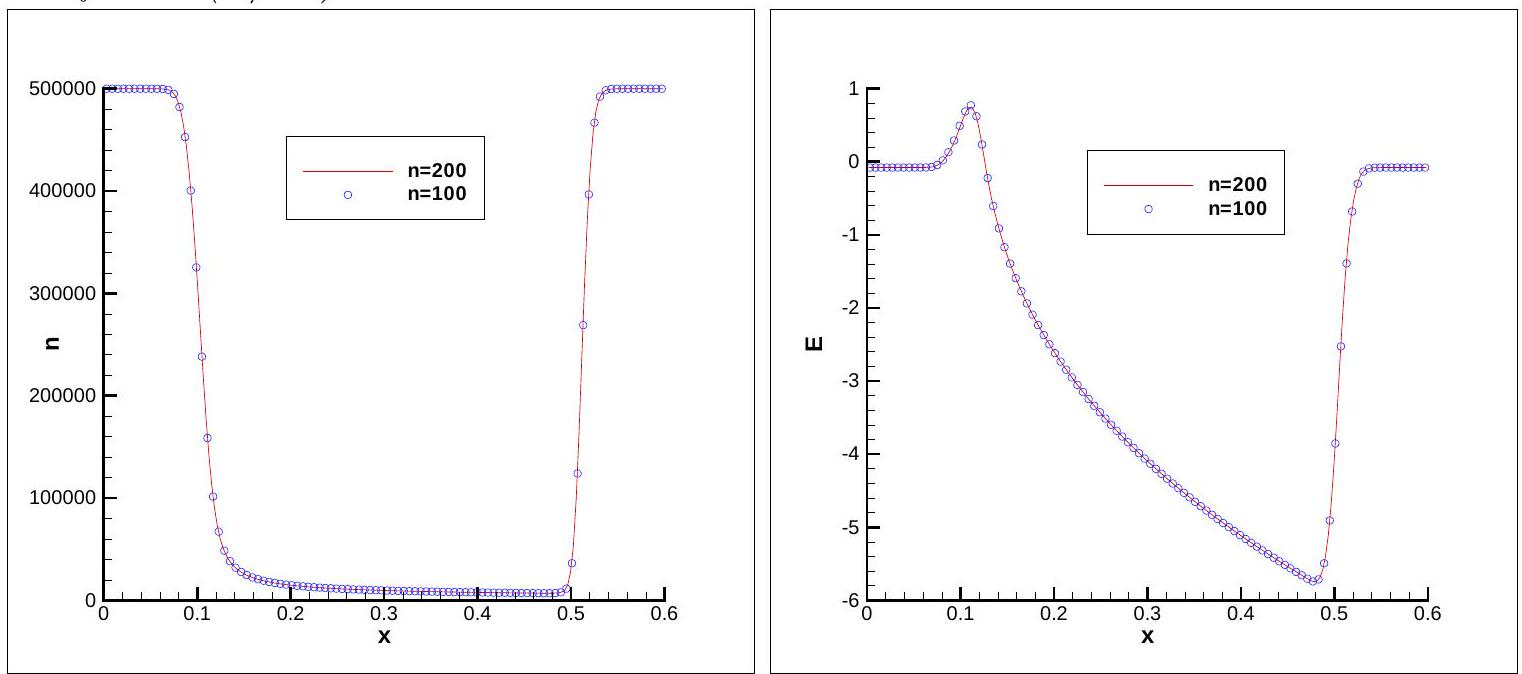
\includegraphics[width=\textwidth]{figure/numbericalsimulationresulttranslation}
    \caption{在 $[0,0.6]$ 有100或200个网格单元, $\Delta t=1.2 E-3$。 左边:密度 $n\left(10^{12} \mathrm{~cm}^{-3}\right)$;右边:电场 $E$ (V/um)。}
    \label{fig:numbericalsimulationresulttranslation}
\end{figure}
\begingroup
\linespreadsingle{}
\printbibliography[title={外文翻译参考文献}]
\endgroup
